% Options for packages loaded elsewhere
\PassOptionsToPackage{unicode}{hyperref}
\PassOptionsToPackage{hyphens}{url}
%
\documentclass[
]{article}
\usepackage{lmodern}
\usepackage{amssymb,amsmath}
\usepackage{ifxetex,ifluatex}
\ifnum 0\ifxetex 1\fi\ifluatex 1\fi=0 % if pdftex
  \usepackage[T1]{fontenc}
  \usepackage[utf8]{inputenc}
  \usepackage{textcomp} % provide euro and other symbols
\else % if luatex or xetex
  \usepackage{unicode-math}
  \defaultfontfeatures{Scale=MatchLowercase}
  \defaultfontfeatures[\rmfamily]{Ligatures=TeX,Scale=1}
\fi
% Use upquote if available, for straight quotes in verbatim environments
\IfFileExists{upquote.sty}{\usepackage{upquote}}{}
\IfFileExists{microtype.sty}{% use microtype if available
  \usepackage[]{microtype}
  \UseMicrotypeSet[protrusion]{basicmath} % disable protrusion for tt fonts
}{}
\makeatletter
\@ifundefined{KOMAClassName}{% if non-KOMA class
  \IfFileExists{parskip.sty}{%
    \usepackage{parskip}
  }{% else
    \setlength{\parindent}{0pt}
    \setlength{\parskip}{6pt plus 2pt minus 1pt}}
}{% if KOMA class
  \KOMAoptions{parskip=half}}
\makeatother
\usepackage{xcolor}
\IfFileExists{xurl.sty}{\usepackage{xurl}}{} % add URL line breaks if available
\IfFileExists{bookmark.sty}{\usepackage{bookmark}}{\usepackage{hyperref}}
\hypersetup{
  pdftitle={Statistical Rethinking 2nd edition Homework 8 in INLA},
  hidelinks,
  pdfcreator={LaTeX via pandoc}}
\urlstyle{same} % disable monospaced font for URLs
\usepackage[margin=1in]{geometry}
\usepackage{color}
\usepackage{fancyvrb}
\newcommand{\VerbBar}{|}
\newcommand{\VERB}{\Verb[commandchars=\\\{\}]}
\DefineVerbatimEnvironment{Highlighting}{Verbatim}{commandchars=\\\{\}}
% Add ',fontsize=\small' for more characters per line
\usepackage{framed}
\definecolor{shadecolor}{RGB}{248,248,248}
\newenvironment{Shaded}{\begin{snugshade}}{\end{snugshade}}
\newcommand{\AlertTok}[1]{\textcolor[rgb]{0.94,0.16,0.16}{#1}}
\newcommand{\AnnotationTok}[1]{\textcolor[rgb]{0.56,0.35,0.01}{\textbf{\textit{#1}}}}
\newcommand{\AttributeTok}[1]{\textcolor[rgb]{0.77,0.63,0.00}{#1}}
\newcommand{\BaseNTok}[1]{\textcolor[rgb]{0.00,0.00,0.81}{#1}}
\newcommand{\BuiltInTok}[1]{#1}
\newcommand{\CharTok}[1]{\textcolor[rgb]{0.31,0.60,0.02}{#1}}
\newcommand{\CommentTok}[1]{\textcolor[rgb]{0.56,0.35,0.01}{\textit{#1}}}
\newcommand{\CommentVarTok}[1]{\textcolor[rgb]{0.56,0.35,0.01}{\textbf{\textit{#1}}}}
\newcommand{\ConstantTok}[1]{\textcolor[rgb]{0.00,0.00,0.00}{#1}}
\newcommand{\ControlFlowTok}[1]{\textcolor[rgb]{0.13,0.29,0.53}{\textbf{#1}}}
\newcommand{\DataTypeTok}[1]{\textcolor[rgb]{0.13,0.29,0.53}{#1}}
\newcommand{\DecValTok}[1]{\textcolor[rgb]{0.00,0.00,0.81}{#1}}
\newcommand{\DocumentationTok}[1]{\textcolor[rgb]{0.56,0.35,0.01}{\textbf{\textit{#1}}}}
\newcommand{\ErrorTok}[1]{\textcolor[rgb]{0.64,0.00,0.00}{\textbf{#1}}}
\newcommand{\ExtensionTok}[1]{#1}
\newcommand{\FloatTok}[1]{\textcolor[rgb]{0.00,0.00,0.81}{#1}}
\newcommand{\FunctionTok}[1]{\textcolor[rgb]{0.00,0.00,0.00}{#1}}
\newcommand{\ImportTok}[1]{#1}
\newcommand{\InformationTok}[1]{\textcolor[rgb]{0.56,0.35,0.01}{\textbf{\textit{#1}}}}
\newcommand{\KeywordTok}[1]{\textcolor[rgb]{0.13,0.29,0.53}{\textbf{#1}}}
\newcommand{\NormalTok}[1]{#1}
\newcommand{\OperatorTok}[1]{\textcolor[rgb]{0.81,0.36,0.00}{\textbf{#1}}}
\newcommand{\OtherTok}[1]{\textcolor[rgb]{0.56,0.35,0.01}{#1}}
\newcommand{\PreprocessorTok}[1]{\textcolor[rgb]{0.56,0.35,0.01}{\textit{#1}}}
\newcommand{\RegionMarkerTok}[1]{#1}
\newcommand{\SpecialCharTok}[1]{\textcolor[rgb]{0.00,0.00,0.00}{#1}}
\newcommand{\SpecialStringTok}[1]{\textcolor[rgb]{0.31,0.60,0.02}{#1}}
\newcommand{\StringTok}[1]{\textcolor[rgb]{0.31,0.60,0.02}{#1}}
\newcommand{\VariableTok}[1]{\textcolor[rgb]{0.00,0.00,0.00}{#1}}
\newcommand{\VerbatimStringTok}[1]{\textcolor[rgb]{0.31,0.60,0.02}{#1}}
\newcommand{\WarningTok}[1]{\textcolor[rgb]{0.56,0.35,0.01}{\textbf{\textit{#1}}}}
\usepackage{graphicx,grffile}
\makeatletter
\def\maxwidth{\ifdim\Gin@nat@width>\linewidth\linewidth\else\Gin@nat@width\fi}
\def\maxheight{\ifdim\Gin@nat@height>\textheight\textheight\else\Gin@nat@height\fi}
\makeatother
% Scale images if necessary, so that they will not overflow the page
% margins by default, and it is still possible to overwrite the defaults
% using explicit options in \includegraphics[width, height, ...]{}
\setkeys{Gin}{width=\maxwidth,height=\maxheight,keepaspectratio}
% Set default figure placement to htbp
\makeatletter
\def\fps@figure{htbp}
\makeatother
\setlength{\emergencystretch}{3em} % prevent overfull lines
\providecommand{\tightlist}{%
  \setlength{\itemsep}{0pt}\setlength{\parskip}{0pt}}
\setcounter{secnumdepth}{-\maxdimen} % remove section numbering

\title{Statistical Rethinking 2nd edition Homework 8 in INLA}
\author{}
\date{\vspace{-2.5em}}

\begin{document}
\maketitle

{
\setcounter{tocdepth}{2}
\tableofcontents
}
\begin{Shaded}
\begin{Highlighting}[]
\KeywordTok{library}\NormalTok{(tidyverse)}
\KeywordTok{library}\NormalTok{(rethinking)}
\KeywordTok{library}\NormalTok{(dagitty)}
\KeywordTok{library}\NormalTok{(INLA)}
\KeywordTok{library}\NormalTok{(knitr)}
\KeywordTok{library}\NormalTok{(stringr)}
\end{Highlighting}
\end{Shaded}

\hypertarget{section}{%
\section{1.}\label{section}}

\textbf{Revisit the Reed frog survival data, data(reedfrogs),and add the
predation and size treatment variables to the varying intercepts model.
Consider models with either predictor alone, both predictors, as well as
a model including their interaction. What do you infer about the causal
influence of these predictor variables? Also focus on the inferred
variation across tanks (the σ across tanks). Explain why it changes as
it does across models with different predictors included.}

\begin{Shaded}
\begin{Highlighting}[]
\KeywordTok{library}\NormalTok{(rethinking) }
\KeywordTok{data}\NormalTok{(reedfrogs)}
\NormalTok{d <-}\StringTok{ }\NormalTok{reedfrogs}
\end{Highlighting}
\end{Shaded}

\hypertarget{varying-intercepts-model}{%
\subsection{1.1 varying intercepts
model}\label{varying-intercepts-model}}

Si ∼ Binomial(Ni, pi)

logit(pi) = αtank{[}i{]}

αj ∼ Normal(\(\bar{\alpha}\), σ) {[}adaptive prior{]}

\(\bar{\alpha}\) ∼ Normal(0, 1.5) {[}prior for average tank{]}

σ ∼ Exponential(1) {[}prior for standard deviation of tanks{]}

\hypertarget{rethinking}{%
\subsubsection{1.1 rethinking}\label{rethinking}}

\begin{Shaded}
\begin{Highlighting}[]
\NormalTok{dat <-}\StringTok{ }\KeywordTok{list}\NormalTok{(}
\DataTypeTok{S =}\NormalTok{ d}\OperatorTok{$}\NormalTok{surv,}
\DataTypeTok{n =}\NormalTok{ d}\OperatorTok{$}\NormalTok{density,}
\DataTypeTok{tank =} \DecValTok{1}\OperatorTok{:}\KeywordTok{nrow}\NormalTok{(d),}
\DataTypeTok{pred =} \KeywordTok{ifelse}\NormalTok{( d}\OperatorTok{$}\NormalTok{pred}\OperatorTok{==}\StringTok{"no"}\NormalTok{ , 0L , 1L ), }
\DataTypeTok{size_ =} \KeywordTok{ifelse}\NormalTok{( d}\OperatorTok{$}\NormalTok{size}\OperatorTok{==}\StringTok{"small"}\NormalTok{ , 1L , 2L )}
\NormalTok{)}
\end{Highlighting}
\end{Shaded}

\begin{Shaded}
\begin{Highlighting}[]
\NormalTok{m1}\FloatTok{.1}\NormalTok{ <-}\StringTok{ }\KeywordTok{ulam}\NormalTok{( }\KeywordTok{alist}\NormalTok{(}
\NormalTok{S }\OperatorTok{~}\StringTok{ }\KeywordTok{binomial}\NormalTok{( n , p ),}
\KeywordTok{logit}\NormalTok{(p) <-}\StringTok{ }\NormalTok{a[tank],}
\NormalTok{a[tank] }\OperatorTok{~}\StringTok{ }\KeywordTok{normal}\NormalTok{( a_bar , sigma ), }
\NormalTok{a_bar }\OperatorTok{~}\StringTok{ }\KeywordTok{normal}\NormalTok{( }\DecValTok{0}\NormalTok{ , }\FloatTok{1.5}\NormalTok{ ),}
\NormalTok{sigma }\OperatorTok{~}\StringTok{ }\KeywordTok{exponential}\NormalTok{( }\DecValTok{1}\NormalTok{ )}
\NormalTok{), }\DataTypeTok{data=}\NormalTok{dat , }\DataTypeTok{chains=}\DecValTok{4}\NormalTok{ , }\DataTypeTok{cores=}\DecValTok{4}\NormalTok{ , }\DataTypeTok{log_lik=}\OtherTok{TRUE}\NormalTok{ )}
\KeywordTok{precis}\NormalTok{(m1}\FloatTok{.1}\NormalTok{, }\DataTypeTok{depth=} \DecValTok{2}\NormalTok{)}
\end{Highlighting}
\end{Shaded}

\begin{verbatim}
##               mean        sd        5.5%       94.5%    n_eff     Rhat4
## a[1]   2.146146420 0.8767432  0.83581149  3.66756437 3686.062 0.9998012
## a[2]   3.102821879 1.1639537  1.43139832  5.10255185 3314.839 1.0001594
## a[3]   1.016279055 0.6697181 -0.01419990  2.14526553 4070.578 0.9981720
## a[4]   3.072400877 1.0736910  1.52935031  4.85895849 2572.300 0.9990339
## a[5]   2.133778161 0.8758528  0.85715411  3.59099602 3563.674 0.9984365
## a[6]   2.145672026 0.8584508  0.88261170  3.64161688 2351.890 0.9995622
## a[7]   3.057364091 1.0524158  1.54262310  4.85741113 2413.757 0.9997951
## a[8]   2.111946340 0.8001730  0.91752077  3.48083521 3248.715 0.9981692
## a[9]  -0.164524596 0.6127761 -1.15216166  0.81019749 3781.126 0.9986917
## a[10]  2.147931123 0.8663970  0.90101946  3.64824503 2011.479 0.9990610
## a[11]  0.998089346 0.6774641 -0.05287242  2.12386212 3167.599 0.9988437
## a[12]  0.589664298 0.6189981 -0.33844485  1.59642964 3153.444 0.9999136
## a[13]  1.021464312 0.6875380 -0.05012920  2.17257412 4540.382 0.9987963
## a[14]  0.182719629 0.6382877 -0.81120105  1.21660676 4916.469 0.9986979
## a[15]  2.147598985 0.9095751  0.79286851  3.69531101 3262.395 0.9991884
## a[16]  2.156564035 0.9038034  0.84583177  3.69778113 2781.057 0.9995792
## a[17]  2.881551949 0.7577498  1.76687039  4.19125375 3276.226 0.9987848
## a[18]  2.403876190 0.6871205  1.38776645  3.56037563 2239.634 0.9989123
## a[19]  2.032265284 0.5807184  1.15002966  3.01571495 2618.076 1.0007672
## a[20]  3.676943489 1.0329977  2.21040957  5.45870117 1920.793 1.0007373
## a[21]  2.384097018 0.6714688  1.36846703  3.54441421 3327.304 0.9999194
## a[22]  2.393418936 0.6503273  1.43812436  3.50092140 2621.390 0.9992413
## a[23]  2.392472646 0.6577443  1.42696113  3.52454765 3378.560 0.9994404
## a[24]  1.704346309 0.5343965  0.87552976  2.58414868 2827.354 0.9997911
## a[25] -1.005856715 0.4699235 -1.78613117 -0.26931675 3681.345 0.9985133
## a[26]  0.159859168 0.3863901 -0.45611184  0.76786372 3864.817 0.9985719
## a[27] -1.442556083 0.4894928 -2.26865360 -0.68088550 2859.885 1.0000096
## a[28] -0.466974346 0.4062470 -1.11345419  0.18377951 5489.128 0.9985114
## a[29]  0.166548590 0.3980811 -0.48110272  0.82158129 4438.917 0.9985477
## a[30]  1.437289676 0.4883911  0.69871697  2.24717464 3452.359 0.9982488
## a[31] -0.631517898 0.4271682 -1.31498415  0.03589381 4654.651 0.9992492
## a[32] -0.310080555 0.4033974 -0.95386569  0.33970300 5005.865 0.9987984
## a[33]  3.196791607 0.7709663  2.08850817  4.51071377 2871.649 0.9989977
## a[34]  2.740150968 0.6589477  1.78280629  3.86539809 2424.795 1.0005928
## a[35]  2.720360589 0.6578902  1.78371920  3.84898127 2469.600 0.9986440
## a[36]  2.064057517 0.5100052  1.30696300  2.92273017 3120.857 0.9987018
## a[37]  2.053374992 0.4804105  1.33246980  2.84210134 3379.426 0.9983884
## a[38]  3.875986412 0.9475825  2.59923226  5.45937589 1783.625 1.0003764
## a[39]  2.696911834 0.6160444  1.77222638  3.74733377 2177.949 1.0020257
## a[40]  2.347097105 0.5466810  1.53999309  3.26674844 3021.844 0.9988599
## a[41] -1.803332879 0.4633261 -2.58701451 -1.09420855 2957.818 0.9994505
## a[42] -0.573228004 0.3318964 -1.12950936 -0.04698206 4053.920 0.9985013
## a[43] -0.452255052 0.3452240 -1.04101168  0.07954403 4381.983 0.9985316
## a[44] -0.341739002 0.3405592 -0.89459101  0.19612685 3868.711 0.9985096
## a[45]  0.576126015 0.3467840  0.03333115  1.13353205 4945.263 0.9987369
## a[46] -0.573540292 0.3617721 -1.15084372 -0.00498894 4149.390 0.9991674
## a[47]  2.067149976 0.5137056  1.28217766  2.90464008 3931.034 0.9989861
## a[48]  0.008435293 0.3202897 -0.48569225  0.51480594 4535.099 0.9984494
## a_bar  1.348583988 0.2563613  0.94400001  1.75191514 2045.778 0.9988849
## sigma  1.618160218 0.2147179  1.30762320  1.99725130 1441.899 1.0001640
\end{verbatim}

\hypertarget{inla}{%
\subsubsection{1.1 INLA}\label{inla}}

following example:
\url{https://people.bath.ac.uk/jjf23/brinla/reeds.html}

\textbf{Here I'm missing custom priors} I'll use a half cauchy prior for
the \(\sigma\) to constrain it to \textgreater0 numbers, which is what
the exponential does as well.

\begin{Shaded}
\begin{Highlighting}[]
\KeywordTok{library}\NormalTok{(brinla)}
\KeywordTok{library}\NormalTok{(INLA)}

\NormalTok{d1.i <-}\StringTok{ }\NormalTok{d }\OperatorTok\StringTok{ }
\StringTok{  }\KeywordTok{mutate}\NormalTok{(}\DataTypeTok{tank =} \KeywordTok{row_number}\NormalTok{(), }
         \DataTypeTok{pred.no=} \KeywordTok{na_if}\NormalTok{(}\KeywordTok{if_else}\NormalTok{(pred}\OperatorTok{==}\StringTok{"no"}\NormalTok{, }\DecValTok{1}\NormalTok{, }\DecValTok{0}\NormalTok{), }\DecValTok{0}\NormalTok{),}
         \DataTypeTok{pred.yes=} \KeywordTok{na_if}\NormalTok{(}\KeywordTok{if_else}\NormalTok{(pred}\OperatorTok{==}\StringTok{"pred"}\NormalTok{, }\DecValTok{1}\NormalTok{, }\DecValTok{0}\NormalTok{), }\DecValTok{0}\NormalTok{),}
         \DataTypeTok{size.small=} \KeywordTok{na_if}\NormalTok{(}\KeywordTok{if_else}\NormalTok{(size}\OperatorTok{==}\StringTok{"small"}\NormalTok{, }\DecValTok{1}\NormalTok{, }\DecValTok{0}\NormalTok{), }\DecValTok{0}\NormalTok{),}
         \DataTypeTok{size.big=} \KeywordTok{na_if}\NormalTok{(}\KeywordTok{if_else}\NormalTok{(size}\OperatorTok{==}\StringTok{"big"}\NormalTok{, }\DecValTok{1}\NormalTok{, }\DecValTok{0}\NormalTok{), }\DecValTok{0}\NormalTok{)}
\NormalTok{         ) }

\CommentTok{# number of trials is d1.i$density}

\NormalTok{halfcauchy =}\StringTok{ "expression:}
\StringTok{              lambda = 0.022;}
\StringTok{              precision = exp(log_precision);}
\StringTok{              logdens = -1.5*log_precision-log(pi*lambda)-log(1+1/(precision*lambda^2));}
\StringTok{              log_jacobian = log_precision;}
\StringTok{              return(logdens+log_jacobian);"}

\NormalTok{hcprior =}\StringTok{ }\KeywordTok{list}\NormalTok{(}\DataTypeTok{prec =} \KeywordTok{list}\NormalTok{(}\DataTypeTok{prior =}\NormalTok{ halfcauchy))}
  
\NormalTok{m1.}\FloatTok{1.}\NormalTok{i <-}\StringTok{ }\KeywordTok{inla}\NormalTok{(surv }\OperatorTok{~}\StringTok{ }\DecValTok{1} \OperatorTok{+}\StringTok{ }\KeywordTok{f}\NormalTok{(tank, }\DataTypeTok{model=}\StringTok{"iid"}\NormalTok{, }\DataTypeTok{hyper =}\NormalTok{ hcprior), }\DataTypeTok{data=}\NormalTok{ d1.i, }\DataTypeTok{family =} \StringTok{"binomial"}\NormalTok{, }
              \DataTypeTok{Ntrials =}\NormalTok{ density, }
              \DataTypeTok{control.family =} \KeywordTok{list}\NormalTok{(}\DataTypeTok{control.link=}\KeywordTok{list}\NormalTok{(}\DataTypeTok{model=}\StringTok{"logit"}\NormalTok{)),}
              \DataTypeTok{control.predictor=}\KeywordTok{list}\NormalTok{(}\DataTypeTok{link=}\DecValTok{1}\NormalTok{, }\DataTypeTok{compute=}\NormalTok{T),}
              \DataTypeTok{control.compute=}\KeywordTok{list}\NormalTok{(}\DataTypeTok{config=}\NormalTok{T, }\DataTypeTok{dic=}\OtherTok{TRUE}\NormalTok{, }\DataTypeTok{waic=} \OtherTok{TRUE}\NormalTok{))}
\KeywordTok{summary}\NormalTok{(m1.}\FloatTok{1.}\NormalTok{i)}
\end{Highlighting}
\end{Shaded}

\begin{verbatim}
## 
## Call:
##    c("inla(formula = surv ~ 1 + f(tank, model = \"iid\", hyper = hcprior), ", " family = \"binomial\", data = d1.i, Ntrials = 
##    density, control.compute = list(config = T, ", " dic = TRUE, waic = TRUE), control.predictor = list(link = 1, ", " compute = T), 
##    control.family = list(control.link = list(model = \"logit\")))" ) 
## Time used:
##     Pre = 1.33, Running = 0.168, Post = 0.202, Total = 1.7 
## Fixed effects:
##             mean    sd 0.025quant 0.5quant 0.975quant  mode kld
## (Intercept) 1.38 0.256       0.89    1.375      1.901 1.364   0
## 
## Random effects:
##   Name     Model
##     tank IID model
## 
## Model hyperparameters:
##                     mean    sd 0.025quant 0.5quant 0.975quant  mode
## Precision for tank 0.415 0.109      0.237    0.404      0.661 0.381
## 
## Expected number of effective parameters(stdev): 40.36(1.26)
## Number of equivalent replicates : 1.19 
## 
## Deviance Information Criterion (DIC) ...............: 214.00
## Deviance Information Criterion (DIC, saturated) ....: 89.62
## Effective number of parameters .....................: 39.50
## 
## Watanabe-Akaike information criterion (WAIC) ...: 205.61
## Effective number of parameters .................: 22.72
## 
## Marginal log-Likelihood:  -140.19 
## Posterior marginals for the linear predictor and
##  the fitted values are computed
\end{verbatim}

\begin{Shaded}
\begin{Highlighting}[]
\NormalTok{m1.}\FloatTok{1.}\NormalTok{i}\OperatorTok{$}\NormalTok{summary.fixed}
\end{Highlighting}
\end{Shaded}

\begin{verbatim}
##                 mean        sd 0.025quant 0.5quant 0.975quant     mode          kld
## (Intercept) 1.380249 0.2562768  0.8904279 1.374944    1.90069 1.364469 1.902443e-05
\end{verbatim}

\begin{Shaded}
\begin{Highlighting}[]
\NormalTok{m1.}\FloatTok{1.}\NormalTok{i}\OperatorTok{$}\NormalTok{summary.hyperpar}
\end{Highlighting}
\end{Shaded}

\begin{verbatim}
##                         mean        sd 0.025quant  0.5quant 0.975quant      mode
## Precision for tank 0.4152469 0.1088217  0.2366839 0.4035007  0.6608823 0.3807222
\end{verbatim}

\begin{Shaded}
\begin{Highlighting}[]
\KeywordTok{bri.hyperpar.summary}\NormalTok{(m1.}\FloatTok{1.}\NormalTok{i)}
\end{Highlighting}
\end{Shaded}

\begin{verbatim}
##                mean        sd   q0.025     q0.5   q0.975     mode
## SD for tank 1.59197 0.2096781 1.231084 1.573964 2.053666 1.539229
\end{verbatim}

it looks like the intercept mean and sd correspond to the
\(\bar{\alpha}\) mean and sd, and the SD for tank corresponds to the
\(\sigma\). this makes sense, because the \(\bar{\alpha}\) is the
average baseline survival for all the tadpoles, which is what the
intercept is. \textbf{BUT I WOULD LOVE IF SOMEONE ELSE CONFIRMED THIS
INTERPRETATION}.

\hypertarget{varying-intercepts-predation}{%
\subsection{1.2 varying intercepts +
predation}\label{varying-intercepts-predation}}

Si ∼ Binomial(Ni, pi)

logit(pi) = αtank{[}i{]} + \(\beta\){[}pred{]}

\(\beta\)∼ Normal(-0.5,1)

αj ∼ Normal(\(\bar{\alpha}\), σ) {[}adaptive prior{]}

\(\bar{\alpha}\) ∼ Normal(0, 1.5) {[}prior for average tank{]}

σ ∼ Exponential(1) {[}prior for standard deviation of tanks{]}

\hypertarget{rethinking-1}{%
\subsubsection{1.2 rethinking}\label{rethinking-1}}

\begin{Shaded}
\begin{Highlighting}[]
\CommentTok{# pred}
\NormalTok{m1}\FloatTok{.2}\NormalTok{ <-}\StringTok{ }\KeywordTok{ulam}\NormalTok{(}
\KeywordTok{alist}\NormalTok{(}
\NormalTok{S }\OperatorTok{~}\StringTok{ }\KeywordTok{binomial}\NormalTok{( n , p ),}
\KeywordTok{logit}\NormalTok{(p) <-}\StringTok{ }\NormalTok{a[tank] }\OperatorTok{+}\StringTok{ }\NormalTok{bp}\OperatorTok{*}\NormalTok{pred, }
\NormalTok{a[tank] }\OperatorTok{~}\StringTok{ }\KeywordTok{normal}\NormalTok{( a_bar , sigma ), }
\NormalTok{bp }\OperatorTok{~}\StringTok{ }\KeywordTok{normal}\NormalTok{( }\FloatTok{-0.5}\NormalTok{ , }\DecValTok{1}\NormalTok{ ),}
\NormalTok{a_bar }\OperatorTok{~}\StringTok{ }\KeywordTok{normal}\NormalTok{( }\DecValTok{0}\NormalTok{ , }\FloatTok{1.5}\NormalTok{ ),}
\NormalTok{sigma }\OperatorTok{~}\StringTok{ }\KeywordTok{exponential}\NormalTok{( }\DecValTok{1}\NormalTok{ )}
\NormalTok{), }\DataTypeTok{data=}\NormalTok{dat , }\DataTypeTok{chains=}\DecValTok{4}\NormalTok{ , }\DataTypeTok{cores=}\DecValTok{4}\NormalTok{ , }\DataTypeTok{log_lik=}\OtherTok{TRUE}\NormalTok{ ) }
\end{Highlighting}
\end{Shaded}

\begin{verbatim}
## Warning: Bulk Effective Samples Size (ESS) is too low, indicating posterior means and medians may be unreliable.
## Running the chains for more iterations may help. See
## http://mc-stan.org/misc/warnings.html#bulk-ess
\end{verbatim}

\begin{Shaded}
\begin{Highlighting}[]
\KeywordTok{precis}\NormalTok{(m1}\FloatTok{.2}\NormalTok{)}
\end{Highlighting}
\end{Shaded}

\begin{verbatim}
##             mean        sd       5.5%     94.5%    n_eff    Rhat4
## bp    -2.4359796 0.2924450 -2.8764198 -1.943438 246.8965 1.005785
## a_bar  2.5331230 0.2279338  2.1692485  2.886476 307.1282 1.004674
## sigma  0.8237866 0.1438996  0.6171576  1.062121 530.1799 1.003489
\end{verbatim}

\hypertarget{inla-1}{%
\subsubsection{1.2 inla}\label{inla-1}}

\begin{Shaded}
\begin{Highlighting}[]
\KeywordTok{library}\NormalTok{(brinla)}
\KeywordTok{library}\NormalTok{(INLA)}

\CommentTok{# number of trials is d1.i$density}

\NormalTok{halfcauchy =}\StringTok{ "expression:}
\StringTok{              lambda = 0.022;}
\StringTok{              precision = exp(log_precision);}
\StringTok{              logdens = -1.5*log_precision-log(pi*lambda)-log(1+1/(precision*lambda^2));}
\StringTok{              log_jacobian = log_precision;}
\StringTok{              return(logdens+log_jacobian);"}

\NormalTok{hcprior =}\StringTok{ }\KeywordTok{list}\NormalTok{(}\DataTypeTok{prec =} \KeywordTok{list}\NormalTok{(}\DataTypeTok{prior =}\NormalTok{ halfcauchy))}
  
\NormalTok{m1.}\FloatTok{2.}\NormalTok{i <-}\StringTok{ }\KeywordTok{inla}\NormalTok{(surv }\OperatorTok{~}\StringTok{ }\DecValTok{1} \OperatorTok{+}\StringTok{ }\NormalTok{pred }\OperatorTok{+}\StringTok{ }\KeywordTok{f}\NormalTok{(tank, }\DataTypeTok{model=}\StringTok{"iid"}\NormalTok{, }\DataTypeTok{hyper =}\NormalTok{ hcprior), }\DataTypeTok{data=}\NormalTok{ d1.i, }\DataTypeTok{family =} \StringTok{"binomial"}\NormalTok{, }
              \DataTypeTok{Ntrials =}\NormalTok{ density, }
              \DataTypeTok{control.fixed =} \KeywordTok{list}\NormalTok{(}
        \DataTypeTok{mean=} \FloatTok{-0.5}\NormalTok{,}
        \DataTypeTok{prec=} \DecValTok{1}\NormalTok{, }
        \DataTypeTok{mean.intercept=} \DecValTok{0}\NormalTok{, }
        \DataTypeTok{prec.intercept=} \DecValTok{1}\OperatorTok{/}\NormalTok{(}\FloatTok{1.5}\OperatorTok{^}\DecValTok{2}\NormalTok{)),}
              \DataTypeTok{control.family =} \KeywordTok{list}\NormalTok{(}\DataTypeTok{control.link=}\KeywordTok{list}\NormalTok{(}\DataTypeTok{model=}\StringTok{"logit"}\NormalTok{)),}
              \DataTypeTok{control.predictor=}\KeywordTok{list}\NormalTok{(}\DataTypeTok{link=}\DecValTok{1}\NormalTok{, }\DataTypeTok{compute=}\NormalTok{T),}
              \DataTypeTok{control.compute=}\KeywordTok{list}\NormalTok{(}\DataTypeTok{config=}\NormalTok{T, }\DataTypeTok{dic=}\OtherTok{TRUE}\NormalTok{, }\DataTypeTok{waic=} \OtherTok{TRUE}\NormalTok{))}
\KeywordTok{summary}\NormalTok{(m1.}\FloatTok{2.}\NormalTok{i)}
\end{Highlighting}
\end{Shaded}

\begin{verbatim}
## 
## Call:
##    c("inla(formula = surv ~ 1 + pred + f(tank, model = \"iid\", hyper = hcprior), ", " family = \"binomial\", data = d1.i, Ntrials = 
##    density, control.compute = list(config = T, ", " dic = TRUE, waic = TRUE), control.predictor = list(link = 1, ", " compute = T), 
##    control.family = list(control.link = list(model = \"logit\")), ", " control.fixed = list(mean = -0.5, prec = 1, mean.intercept = 
##    0, ", " prec.intercept = 1/(1.5^2)))") 
## Time used:
##     Pre = 1.42, Running = 0.199, Post = 0.217, Total = 1.83 
## Fixed effects:
##               mean    sd 0.025quant 0.5quant 0.975quant   mode kld
## (Intercept)  2.523 0.225      2.088    2.520      2.974  2.515   0
## predpred    -2.435 0.288     -2.997   -2.437     -1.863 -2.440   0
## 
## Random effects:
##   Name     Model
##     tank IID model
## 
## Model hyperparameters:
##                    mean    sd 0.025quant 0.5quant 0.975quant mode
## Precision for tank 1.80 0.677       0.85     1.68       3.46 1.48
## 
## Expected number of effective parameters(stdev): 28.98(3.36)
## Number of equivalent replicates : 1.66 
## 
## Deviance Information Criterion (DIC) ...............: 204.42
## Deviance Information Criterion (DIC, saturated) ....: 79.99
## Effective number of parameters .....................: 29.04
## 
## Watanabe-Akaike information criterion (WAIC) ...: 201.45
## Effective number of parameters .................: 19.59
## 
## Marginal log-Likelihood:  -122.10 
## Posterior marginals for the linear predictor and
##  the fitted values are computed
\end{verbatim}

\begin{Shaded}
\begin{Highlighting}[]
\NormalTok{m1.}\FloatTok{2.}\NormalTok{i}\OperatorTok{$}\NormalTok{summary.fixed}
\end{Highlighting}
\end{Shaded}

\begin{verbatim}
##                  mean        sd 0.025quant  0.5quant 0.975quant      mode          kld
## (Intercept)  2.523164 0.2252490   2.087742  2.520414   2.974171  2.514827 2.391528e-07
## predpred    -2.435197 0.2876891  -2.996768 -2.437046  -1.863173 -2.440294 8.877976e-07
\end{verbatim}

\begin{Shaded}
\begin{Highlighting}[]
\KeywordTok{bri.hyperpar.summary}\NormalTok{(m1.}\FloatTok{2.}\NormalTok{i)}
\end{Highlighting}
\end{Shaded}

\begin{verbatim}
##                  mean        sd    q0.025      q0.5   q0.975      mode
## SD for tank 0.7815832 0.1385647 0.5384615 0.7711308 1.082806 0.7517625
\end{verbatim}

\hypertarget{varying-intercepts-size}{%
\subsection{1.3 varying intercepts +
size}\label{varying-intercepts-size}}

Si ∼ Binomial(Ni, pi)

logit(pi) = αtank{[}i{]} + \(\beta\)size

\(\beta\)∼ Normal(0 , 0.5 ) αj ∼ Normal(\(\bar{\alpha}\), σ) {[}adaptive
prior{]}

\(\bar{\alpha}\) ∼ Normal(0, 1.5) {[}prior for average tank{]}

σ ∼ Exponential(1) {[}prior for standard deviation of tanks{]}

\hypertarget{rethinking-2}{%
\subsubsection{1.3 rethinking}\label{rethinking-2}}

\begin{Shaded}
\begin{Highlighting}[]
\KeywordTok{library}\NormalTok{(rethinking) }
\KeywordTok{data}\NormalTok{(reedfrogs)}
\NormalTok{d <-}\StringTok{ }\NormalTok{reedfrogs}

\CommentTok{# size}
\NormalTok{m1}\FloatTok{.3}\NormalTok{ <-}\StringTok{ }\KeywordTok{ulam}\NormalTok{( }\KeywordTok{alist}\NormalTok{(}
\NormalTok{S }\OperatorTok{~}\StringTok{ }\KeywordTok{binomial}\NormalTok{( n , p ),}
\KeywordTok{logit}\NormalTok{(p) <-}\StringTok{ }\NormalTok{a[tank] }\OperatorTok{+}\StringTok{ }\NormalTok{s[size_], }
\NormalTok{a[tank] }\OperatorTok{~}\StringTok{ }\KeywordTok{normal}\NormalTok{( a_bar , sigma ), }
\NormalTok{s[size_] }\OperatorTok{~}\StringTok{ }\KeywordTok{normal}\NormalTok{( }\DecValTok{0}\NormalTok{ , }\FloatTok{0.5}\NormalTok{ ), }
\NormalTok{a_bar }\OperatorTok{~}\StringTok{ }\KeywordTok{normal}\NormalTok{( }\DecValTok{0}\NormalTok{ , }\FloatTok{1.5}\NormalTok{ ),}
\NormalTok{sigma }\OperatorTok{~}\StringTok{ }\KeywordTok{exponential}\NormalTok{( }\DecValTok{1}\NormalTok{ )}
\NormalTok{), }\DataTypeTok{data=}\NormalTok{dat , }\DataTypeTok{chains=}\DecValTok{4}\NormalTok{ , }\DataTypeTok{cores=}\DecValTok{4}\NormalTok{ , }\DataTypeTok{log_lik=}\OtherTok{TRUE}\NormalTok{ )}
\end{Highlighting}
\end{Shaded}

\begin{verbatim}
## Warning: Bulk Effective Samples Size (ESS) is too low, indicating posterior means and medians may be unreliable.
## Running the chains for more iterations may help. See
## http://mc-stan.org/misc/warnings.html#bulk-ess
\end{verbatim}

\begin{verbatim}
## Warning: Tail Effective Samples Size (ESS) is too low, indicating posterior variances and tail quantiles may be unreliable.
## Running the chains for more iterations may help. See
## http://mc-stan.org/misc/warnings.html#tail-ess
\end{verbatim}

\begin{Shaded}
\begin{Highlighting}[]
\KeywordTok{precis}\NormalTok{(m1}\FloatTok{.3}\NormalTok{,  }\DataTypeTok{depth=}\DecValTok{2}\NormalTok{)}
\end{Highlighting}
\end{Shaded}

\begin{verbatim}
##               mean        sd       5.5%       94.5%    n_eff     Rhat4
## a[1]   2.165625815 0.9401077  0.7453984  3.75033152 760.8554 0.9989825
## a[2]   3.043833499 1.1352846  1.3356060  4.98841538 905.8433 1.0003340
## a[3]   1.025976337 0.7826817 -0.2152537  2.30889225 455.4755 1.0027820
## a[4]   3.032761845 1.1384806  1.3549807  5.02260295 948.3125 1.0005022
## a[5]   1.934144115 0.9862191  0.4792170  3.59986533 894.0600 1.0035426
## a[6]   1.937889268 0.9230881  0.5207736  3.47387724 771.3866 1.0042185
## a[7]   2.878734810 1.1805476  1.2239099  4.91035481 904.7830 0.9999333
## a[8]   1.958069563 0.9504631  0.5383716  3.54947916 705.0968 1.0000815
## a[9]  -0.151847926 0.7182937 -1.3195677  0.96795134 510.6954 1.0024445
## a[10]  2.145281672 0.9409965  0.7256978  3.75612951 668.0499 1.0021948
## a[11]  1.047041769 0.7935325 -0.2231269  2.32321657 557.4818 1.0032078
## a[12]  0.619405692 0.7479413 -0.5026785  1.84802357 486.2868 1.0046667
## a[13]  0.800652126 0.7691433 -0.3810980  1.99936901 572.0768 1.0014096
## a[14] -0.003771841 0.7057758 -1.1431189  1.13370602 693.6154 1.0004677
## a[15]  1.937295140 0.9528793  0.5101752  3.55782916 894.7650 1.0023001
## a[16]  1.948871032 0.9351210  0.5474121  3.52137965 826.4943 1.0034344
## a[17]  2.938977210 0.8466007  1.6314357  4.39754094 387.1043 1.0025021
## a[18]  2.453557005 0.7903554  1.2519086  3.79946055 580.5923 1.0027024
## a[19]  2.053448584 0.7373131  0.9423064  3.25279081 519.6057 1.0018668
## a[20]  3.704338922 1.0741377  2.1373529  5.59857592 786.3449 1.0011748
## a[21]  2.170212810 0.7457020  1.0464477  3.44076499 682.1129 1.0008636
## a[22]  2.189338742 0.7716077  1.0592665  3.49757133 725.1988 1.0029454
## a[23]  2.194353009 0.7823092  1.0373155  3.51355462 736.1801 1.0023706
## a[24]  1.466294804 0.6573087  0.4437921  2.58080938 622.9437 1.0043703
## a[25] -0.953501376 0.5888834 -1.9122445 -0.04370461 329.1308 1.0063719
## a[26]  0.204984505 0.5709450 -0.6924557  1.12653247 289.8942 1.0082488
## a[27] -1.396006567 0.6531701 -2.4703891 -0.36679280 371.3134 1.0069940
## a[28] -0.418860426 0.5688968 -1.3395020  0.44668765 331.0422 1.0021341
## a[29] -0.067476349 0.5496244 -0.9490604  0.80161170 485.3129 1.0020249
## a[30]  1.213516170 0.6141342  0.2511470  2.21017292 594.7968 1.0036055
## a[31] -0.875501655 0.5364046 -1.7391601 -0.01454111 422.1074 1.0024841
## a[32] -0.542633375 0.5387474 -1.3993261  0.33382467 441.3826 1.0014640
## a[33]  3.214107521 0.8250856  2.0026118  4.60092062 590.7385 1.0061570
## a[34]  2.743478576 0.7617808  1.6239039  4.03971158 519.0805 1.0010846
## a[35]  2.754179861 0.7832820  1.5936300  4.07672242 521.8480 1.0033397
## a[36]  2.091133378 0.6546110  1.1056138  3.19083831 400.5363 1.0028970
## a[37]  1.833124298 0.6576910  0.8582707  2.94908835 527.2522 1.0028036
## a[38]  3.732630439 1.0700647  2.1494665  5.60772318 850.9455 0.9998256
## a[39]  2.504778418 0.7597139  1.3414309  3.74537798 598.2672 1.0031775
## a[40]  2.122732469 0.6756724  1.0995245  3.22553376 594.1984 1.0021276
## a[41] -1.765600264 0.6246589 -2.7682434 -0.78995520 330.3545 1.0041288
## a[42] -0.513718084 0.5251409 -1.3770373  0.30788390 290.1691 1.0046313
## a[43] -0.398622046 0.5396416 -1.2776235  0.43537740 291.2980 1.0052785
## a[44] -0.283594322 0.5422688 -1.1676802  0.58509471 269.7985 1.0098589
## a[45]  0.354907592 0.5268930 -0.5028190  1.18602550 390.1384 1.0056458
## a[46] -0.802318210 0.5283453 -1.6888835  0.03060874 460.9889 1.0045079
## a[47]  1.830110251 0.6476969  0.8255687  2.89492995 595.8416 1.0056051
## a[48] -0.240316638 0.5037696 -1.0157755  0.57877691 390.2596 1.0045426
## s[1]   0.235274487 0.3837453 -0.3994758  0.86682979 241.8949 1.0076540
## s[2]  -0.054222988 0.4059064 -0.6753943  0.61008139 191.6131 1.0101241
## a_bar  1.254744064 0.4175182  0.5956289  1.91219187 253.7277 1.0044734
## sigma  1.614091032 0.2159493  1.3186804  1.99653510 896.2248 0.9996464
\end{verbatim}

\hypertarget{inla-2}{%
\subsubsection{1.3 inla}\label{inla-2}}

\begin{Shaded}
\begin{Highlighting}[]
\KeywordTok{library}\NormalTok{(brinla)}
\KeywordTok{library}\NormalTok{(INLA)}
\KeywordTok{library}\NormalTok{(tidyverse)}

\NormalTok{d1.i <-}\StringTok{ }\NormalTok{d }\OperatorTok\StringTok{ }
\StringTok{  }\KeywordTok{mutate}\NormalTok{(}\DataTypeTok{tank =} \KeywordTok{row_number}\NormalTok{(), }
         \DataTypeTok{pred.no=} \KeywordTok{na_if}\NormalTok{(}\KeywordTok{if_else}\NormalTok{(pred}\OperatorTok{==}\StringTok{"no"}\NormalTok{, }\DecValTok{1}\NormalTok{, }\DecValTok{0}\NormalTok{), }\DecValTok{0}\NormalTok{),}
         \DataTypeTok{pred.yes=} \KeywordTok{na_if}\NormalTok{(}\KeywordTok{if_else}\NormalTok{(pred}\OperatorTok{==}\StringTok{"pred"}\NormalTok{, }\DecValTok{1}\NormalTok{, }\DecValTok{0}\NormalTok{), }\DecValTok{0}\NormalTok{),}
         \DataTypeTok{size.small=} \KeywordTok{na_if}\NormalTok{(}\KeywordTok{if_else}\NormalTok{(size}\OperatorTok{==}\StringTok{"small"}\NormalTok{, }\DecValTok{1}\NormalTok{, }\DecValTok{0}\NormalTok{), }\DecValTok{0}\NormalTok{),}
         \DataTypeTok{size.big=} \KeywordTok{na_if}\NormalTok{(}\KeywordTok{if_else}\NormalTok{(size}\OperatorTok{==}\StringTok{"big"}\NormalTok{, }\DecValTok{1}\NormalTok{, }\DecValTok{0}\NormalTok{), }\DecValTok{0}\NormalTok{)}
\NormalTok{         ) }

\CommentTok{# number of trials is d1.i$density}

\NormalTok{halfcauchy =}\StringTok{ "expression:}
\StringTok{              lambda = 0.022;}
\StringTok{              precision = exp(log_precision);}
\StringTok{              logdens = -1.5*log_precision-log(pi*lambda)-log(1+1/(precision*lambda^2));}
\StringTok{              log_jacobian = log_precision;}
\StringTok{              return(logdens+log_jacobian);"}

\NormalTok{hcprior =}\StringTok{ }\KeywordTok{list}\NormalTok{(}\DataTypeTok{prec =} \KeywordTok{list}\NormalTok{(}\DataTypeTok{prior =}\NormalTok{ halfcauchy))}
  
\NormalTok{m1.}\FloatTok{3.}\NormalTok{i <-}\StringTok{ }\KeywordTok{inla}\NormalTok{(surv }\OperatorTok{~}\StringTok{ }\DecValTok{1} \OperatorTok{+}\StringTok{ }\NormalTok{size.small}\OperatorTok{+}\StringTok{ }\NormalTok{size.big }\OperatorTok{+}\StringTok{ }\KeywordTok{f}\NormalTok{(tank, }\DataTypeTok{model=}\StringTok{"iid"}\NormalTok{, }\DataTypeTok{hyper =}\NormalTok{ hcprior), }\DataTypeTok{data=}\NormalTok{ d1.i, }\DataTypeTok{family =} \StringTok{"binomial"}\NormalTok{, }
              \DataTypeTok{Ntrials =}\NormalTok{ density, }
              \DataTypeTok{control.fixed =} \KeywordTok{list}\NormalTok{(}
        \DataTypeTok{mean=} \DecValTok{0}\NormalTok{,}
        \DataTypeTok{prec=} \DecValTok{1}\OperatorTok{/}\NormalTok{(}\FloatTok{0.5}\OperatorTok{^}\DecValTok{2}\NormalTok{), }
        \DataTypeTok{mean.intercept=} \DecValTok{0}\NormalTok{, }
        \DataTypeTok{prec.intercept=} \DecValTok{1}\OperatorTok{/}\NormalTok{(}\FloatTok{1.5}\OperatorTok{^}\DecValTok{2}\NormalTok{)),}
              \DataTypeTok{control.family =} \KeywordTok{list}\NormalTok{(}\DataTypeTok{control.link=}\KeywordTok{list}\NormalTok{(}\DataTypeTok{model=}\StringTok{"logit"}\NormalTok{)),}
              \DataTypeTok{control.predictor=}\KeywordTok{list}\NormalTok{(}\DataTypeTok{link=}\DecValTok{1}\NormalTok{, }\DataTypeTok{compute=}\NormalTok{T),}
              \DataTypeTok{control.compute=}\KeywordTok{list}\NormalTok{(}\DataTypeTok{config=}\NormalTok{T, }\DataTypeTok{dic=}\OtherTok{TRUE}\NormalTok{, }\DataTypeTok{waic=} \OtherTok{TRUE}\NormalTok{))}
\KeywordTok{summary}\NormalTok{(m1.}\FloatTok{3.}\NormalTok{i)}
\end{Highlighting}
\end{Shaded}

\begin{verbatim}
## 
## Call:
##    c("inla(formula = surv ~ 1 + size.small + size.big + f(tank, model = \"iid\", ", " hyper = hcprior), family = \"binomial\", data = 
##    d1.i, Ntrials = density, ", " control.compute = list(config = T, dic = TRUE, waic = TRUE), ", " control.predictor = list(link = 1, 
##    compute = T), control.family = list(control.link = list(model = \"logit\")), ", " control.fixed = list(mean = 0, prec = 1/(0.5^2), 
##    mean.intercept = 0, ", " prec.intercept = 1/(1.5^2)))") 
## Time used:
##     Pre = 1.47, Running = 0.185, Post = 0.224, Total = 1.88 
## Fixed effects:
##               mean    sd 0.025quant 0.5quant 0.975quant   mode kld
## (Intercept)  1.272 0.418      0.455    1.271      2.095  1.268   0
## size.small   0.222 0.400     -0.564    0.223      1.007  0.223   0
## size.big    -0.081 0.400     -0.866   -0.082      0.705 -0.082   0
## 
## Random effects:
##   Name     Model
##     tank IID model
## 
## Model hyperparameters:
##                     mean    sd 0.025quant 0.5quant 0.975quant  mode
## Precision for tank 0.421 0.111      0.239    0.408      0.672 0.385
## 
## Expected number of effective parameters(stdev): 40.42(1.26)
## Number of equivalent replicates : 1.19 
## 
## Deviance Information Criterion (DIC) ...............: 214.43
## Deviance Information Criterion (DIC, saturated) ....: 90.04
## Effective number of parameters .....................: 39.58
## 
## Watanabe-Akaike information criterion (WAIC) ...: 206.21
## Effective number of parameters .................: 22.90
## 
## Marginal log-Likelihood:  -142.21 
## Posterior marginals for the linear predictor and
##  the fitted values are computed
\end{verbatim}

\begin{Shaded}
\begin{Highlighting}[]
\NormalTok{m1.}\FloatTok{3.}\NormalTok{i}\OperatorTok{$}\NormalTok{summary.fixed}
\end{Highlighting}
\end{Shaded}

\begin{verbatim}
##                    mean        sd 0.025quant    0.5quant 0.975quant       mode          kld
## (Intercept)  1.27186665 0.4177740  0.4549238  1.27059867   2.095210  1.2681232 2.406671e-06
## size.small   0.22245891 0.4001376 -0.5640040  0.22269633   1.006898  0.2232035 1.123068e-07
## size.big    -0.08147702 0.4002655 -0.8664804 -0.08182627   0.704788 -0.0824901 6.786554e-07
\end{verbatim}

\begin{Shaded}
\begin{Highlighting}[]
\KeywordTok{bri.hyperpar.summary}\NormalTok{(m1.}\FloatTok{3.}\NormalTok{i)}
\end{Highlighting}
\end{Shaded}

\begin{verbatim}
##                 mean        sd   q0.025    q0.5   q0.975     mode
## SD for tank 1.582503 0.2100774 1.220948 1.56446 2.045071 1.529635
\end{verbatim}

\hypertarget{varying-intercepts-predation-size}{%
\subsection{1.4 varying intercepts + predation +
size}\label{varying-intercepts-predation-size}}

Si ∼ Binomial(Ni, pi)

logit(pi) = αtank{[}i{]} + \(\beta\)size + \(\gamma\)size

\(\gamma\) ∼ Normal(0 , 0.5)

\(\beta\) ∼ Normal(-0.5,1) αj ∼ Normal(\(\bar{\alpha}\), σ) {[}adaptive
prior{]}

\(\bar{\alpha}\) ∼ Normal(0, 1.5) {[}prior for average tank{]}

σ ∼ Exponential(1) {[}prior for standard deviation of tanks{]}

\hypertarget{rethinking-3}{%
\subsubsection{1.4 rethinking}\label{rethinking-3}}

\begin{Shaded}
\begin{Highlighting}[]
\CommentTok{# pred + size }
\NormalTok{m1}\FloatTok{.4}\NormalTok{ <-}\StringTok{ }\KeywordTok{ulam}\NormalTok{(}
\KeywordTok{alist}\NormalTok{(}
\NormalTok{S }\OperatorTok{~}\StringTok{ }\KeywordTok{binomial}\NormalTok{( n , p ),}
\KeywordTok{logit}\NormalTok{(p) <-}\StringTok{ }\NormalTok{a[tank] }\OperatorTok{+}\StringTok{ }\NormalTok{bp}\OperatorTok{*}\NormalTok{pred }\OperatorTok{+}\StringTok{ }\NormalTok{s[size_], }
\NormalTok{a[tank] }\OperatorTok{~}\StringTok{ }\KeywordTok{normal}\NormalTok{( a_bar , sigma ),}
\NormalTok{bp }\OperatorTok{~}\StringTok{ }\KeywordTok{normal}\NormalTok{( }\FloatTok{-0.5}\NormalTok{ , }\DecValTok{1}\NormalTok{ ),}
\NormalTok{s[size_] }\OperatorTok{~}\StringTok{ }\KeywordTok{normal}\NormalTok{( }\DecValTok{0}\NormalTok{ , }\FloatTok{0.5}\NormalTok{ ),}
\NormalTok{a_bar }\OperatorTok{~}\StringTok{ }\KeywordTok{normal}\NormalTok{( }\DecValTok{0}\NormalTok{ , }\FloatTok{1.5}\NormalTok{ ),}
\NormalTok{sigma }\OperatorTok{~}\StringTok{ }\KeywordTok{exponential}\NormalTok{( }\DecValTok{1}\NormalTok{ )}
\NormalTok{), }\DataTypeTok{data=}\NormalTok{dat , }\DataTypeTok{chains=}\DecValTok{4}\NormalTok{ , }\DataTypeTok{cores=}\DecValTok{4}\NormalTok{ , }\DataTypeTok{log_lik=}\OtherTok{TRUE}\NormalTok{ )}
\end{Highlighting}
\end{Shaded}

\begin{verbatim}
## Warning: Bulk Effective Samples Size (ESS) is too low, indicating posterior means and medians may be unreliable.
## Running the chains for more iterations may help. See
## http://mc-stan.org/misc/warnings.html#bulk-ess
\end{verbatim}

\begin{verbatim}
## Warning: Tail Effective Samples Size (ESS) is too low, indicating posterior variances and tail quantiles may be unreliable.
## Running the chains for more iterations may help. See
## http://mc-stan.org/misc/warnings.html#tail-ess
\end{verbatim}

\begin{Shaded}
\begin{Highlighting}[]
\KeywordTok{precis}\NormalTok{(m1}\FloatTok{.4}\NormalTok{, }\DataTypeTok{depth=}\DecValTok{2}\NormalTok{)}
\end{Highlighting}
\end{Shaded}

\begin{verbatim}
##             mean        sd         5.5%      94.5%    n_eff     Rhat4
## a[1]   2.4731049 0.7640641  1.291247189  3.7552403 384.6247 1.0050219
## a[2]   2.8645084 0.7859337  1.702271570  4.1816970 407.1706 1.0037451
## a[3]   1.7307311 0.7142943  0.591788966  2.8435771 383.1317 1.0069170
## a[4]   2.8767173 0.8100380  1.644100563  4.2271239 403.5257 1.0026720
## a[5]   2.3234035 0.7802774  1.105071941  3.5481647 483.4486 1.0037271
## a[6]   2.3213359 0.7850950  1.085379690  3.6334987 395.7219 1.0069757
## a[7]   2.7710256 0.8120282  1.538302467  4.0913109 502.8185 1.0012895
## a[8]   2.3368783 0.7847429  1.102765489  3.6209030 430.7275 1.0051122
## a[9]   2.2659487 0.6669266  1.216406382  3.3013650 294.1751 1.0087116
## a[10]  3.5228454 0.7132831  2.420747573  4.6650555 307.2647 1.0084048
## a[11]  3.0000206 0.6787343  1.927139066  4.1138684 276.6105 1.0096751
## a[12]  2.7284252 0.6823338  1.661071437  3.8456377 273.7623 1.0121084
## a[13]  2.7565388 0.6717392  1.689312274  3.8454026 294.0144 1.0094230
## a[14]  2.2419150 0.6672728  1.171453717  3.3573047 297.4462 1.0070679
## a[15]  3.3072058 0.7214197  2.176795683  4.4976522 349.0866 1.0050565
## a[16]  3.3132558 0.7066483  2.206949874  4.4540690 325.8577 1.0095233
## a[17]  2.8636684 0.7127265  1.774124324  4.0108647 379.4747 1.0072866
## a[18]  2.5617566 0.6682614  1.540732010  3.6289877 367.9755 1.0055719
## a[19]  2.2954859 0.6309834  1.301217131  3.3288938 335.1825 1.0050726
## a[20]  3.1984258 0.7572131  2.000720914  4.4750622 372.5104 1.0067998
## a[21]  2.3181974 0.6549116  1.291781560  3.3501989 366.9632 1.0064968
## a[22]  2.3446333 0.6927057  1.276329704  3.4949406 427.3130 1.0031171
## a[23]  2.3520719 0.6612198  1.332027346  3.3952867 347.7979 1.0052444
## a[24]  1.7901049 0.6469469  0.748856470  2.8199141 333.5010 1.0061050
## a[25]  1.6447074 0.6089402  0.650879945  2.6480372 232.1878 1.0130821
## a[26]  2.5814090 0.6018691  1.628702281  3.5566090 219.3323 1.0105023
## a[27]  1.3508752 0.6394872  0.354435773  2.3852357 254.3691 1.0106334
## a[28]  2.0706590 0.5867767  1.118343296  3.0210910 219.8050 1.0134103
## a[29]  2.2381865 0.5878211  1.326178428  3.1706935 244.3672 1.0102909
## a[30]  3.2211837 0.6226819  2.271857863  4.2467480 241.2802 1.0113797
## a[31]  1.5997886 0.5817788  0.663024242  2.5385352 227.8722 1.0134596
## a[32]  1.8721253 0.5925444  0.910370686  2.8224682 232.7031 1.0139492
## a[33]  3.0300862 0.6612918  2.035337164  4.1142494 322.3832 1.0052705
## a[34]  2.7807457 0.6667142  1.781573062  3.9218535 337.0857 1.0079014
## a[35]  2.7557250 0.6342874  1.792322152  3.7650569 357.6986 1.0051182
## a[36]  2.3096005 0.6197722  1.346417366  3.3012877 300.3912 1.0086087
## a[37]  2.0336566 0.6173676  1.074611165  3.0680948 302.9369 1.0074491
## a[38]  3.1687149 0.7660233  2.015819715  4.4800640 382.3226 1.0048680
## a[39]  2.5219222 0.6478632  1.497926360  3.5534773 333.9128 1.0080721
## a[40]  2.2683422 0.6351588  1.279785548  3.3033528 350.1712 1.0028275
## a[41]  1.0208398 0.6300785 -0.002296373  2.0211963 251.5370 1.0088974
## a[42]  1.9845863 0.5925185  1.020235224  2.9282234 218.9073 1.0125133
## a[43]  2.0911992 0.5766688  1.168039957  3.0174978 209.7759 1.0145584
## a[44]  2.1912019 0.5849320  1.284673074  3.1413162 216.4067 1.0114954
## a[45]  2.6167814 0.5754486  1.746000414  3.5772125 211.9483 1.0151165
## a[46]  1.6288690 0.5760375  0.721259261  2.5286852 214.1787 1.0123990
## a[47]  3.6993574 0.6182008  2.707207964  4.7162247 236.4413 1.0155590
## a[48]  2.1380254 0.5759534  1.245311382  3.0686365 218.8263 1.0143556
## bp    -2.4448434 0.2867734 -2.901053361 -1.9720788 639.6620 1.0062691
## s[1]   0.3267422 0.3872068 -0.283926000  0.9341774 180.6016 1.0127086
## s[2]  -0.1137287 0.3968376 -0.735165279  0.5056111 176.9722 1.0156026
## a_bar  2.4322349 0.4362440  1.773457404  3.1540356 144.8045 1.0191983
## sigma  0.7751090 0.1399293  0.566003195  1.0099085 626.2910 0.9999478
\end{verbatim}

\hypertarget{inla-3}{%
\subsubsection{1.4 inla}\label{inla-3}}

\begin{Shaded}
\begin{Highlighting}[]
\KeywordTok{library}\NormalTok{(brinla)}
\KeywordTok{library}\NormalTok{(INLA)}

\CommentTok{# number of trials is d1.i$density}

\NormalTok{halfcauchy =}\StringTok{ "expression:}
\StringTok{              lambda = 0.022;}
\StringTok{              precision = exp(log_precision);}
\StringTok{              logdens = -1.5*log_precision-log(pi*lambda)-log(1+1/(precision*lambda^2));}
\StringTok{              log_jacobian = log_precision;}
\StringTok{              return(logdens+log_jacobian);"}

\NormalTok{hcprior =}\StringTok{ }\KeywordTok{list}\NormalTok{(}\DataTypeTok{prec =} \KeywordTok{list}\NormalTok{(}\DataTypeTok{prior =}\NormalTok{ halfcauchy))}
  
\NormalTok{m1.}\FloatTok{4.}\NormalTok{i <-}\StringTok{ }\KeywordTok{inla}\NormalTok{(surv }\OperatorTok{~}\StringTok{ }\DecValTok{1} \OperatorTok{+}\StringTok{ }\NormalTok{pred }\OperatorTok{+}\StringTok{ }\NormalTok{size.small}\OperatorTok{+}\StringTok{ }\NormalTok{size.big }\OperatorTok{+}\StringTok{ }\KeywordTok{f}\NormalTok{(tank, }\DataTypeTok{model=}\StringTok{"iid"}\NormalTok{, }\DataTypeTok{hyper =}\NormalTok{ hcprior), }\DataTypeTok{data=}\NormalTok{ d1.i, }\DataTypeTok{family =} \StringTok{"binomial"}\NormalTok{, }
              \DataTypeTok{Ntrials =}\NormalTok{ density, }
              \DataTypeTok{control.fixed =} \KeywordTok{list}\NormalTok{(}
        \DataTypeTok{mean=} \KeywordTok{list}\NormalTok{(}\DataTypeTok{pred=} \FloatTok{-0.5}\NormalTok{,}\DataTypeTok{size.small=} \DecValTok{0}\NormalTok{, }\DataTypeTok{size.big=} \DecValTok{0}\NormalTok{ ),}
        \DataTypeTok{prec=} \KeywordTok{list}\NormalTok{(}\DataTypeTok{pred=} \DecValTok{1}\NormalTok{,}\DataTypeTok{size.small=} \DecValTok{1}\NormalTok{, }\DataTypeTok{size.big=} \DecValTok{1}\NormalTok{ ), }
        \DataTypeTok{mean.intercept=} \DecValTok{0}\NormalTok{, }
        \DataTypeTok{prec.intercept=} \DecValTok{1}\OperatorTok{/}\NormalTok{(}\FloatTok{1.5}\OperatorTok{^}\DecValTok{2}\NormalTok{)),}
              \DataTypeTok{control.family =} \KeywordTok{list}\NormalTok{(}\DataTypeTok{control.link=}\KeywordTok{list}\NormalTok{(}\DataTypeTok{model=}\StringTok{"logit"}\NormalTok{)),}
              \DataTypeTok{control.predictor=}\KeywordTok{list}\NormalTok{(}\DataTypeTok{link=}\DecValTok{1}\NormalTok{, }\DataTypeTok{compute=}\NormalTok{T),}
              \DataTypeTok{control.compute=}\KeywordTok{list}\NormalTok{(}\DataTypeTok{config=}\NormalTok{T, }\DataTypeTok{dic=}\OtherTok{TRUE}\NormalTok{, }\DataTypeTok{waic=} \OtherTok{TRUE}\NormalTok{))}
\KeywordTok{summary}\NormalTok{(m1.}\FloatTok{4.}\NormalTok{i)}
\end{Highlighting}
\end{Shaded}

\begin{verbatim}
## 
## Call:
##    c("inla(formula = surv ~ 1 + pred + size.small + size.big + f(tank, ", " model = \"iid\", hyper = hcprior), family = \"binomial\", 
##    data = d1.i, ", " Ntrials = density, control.compute = list(config = T, dic = TRUE, ", " waic = TRUE), control.predictor = 
##    list(link = 1, compute = T), ", " control.family = list(control.link = list(model = \"logit\")), ", " control.fixed = list(mean = 
##    list(pred = -0.5, size.small = 0, ", " size.big = 0), prec = list(pred = 1, size.small = 1, ", " size.big = 1), mean.intercept = 
##    0, prec.intercept = 1/(1.5^2)))" ) 
## Time used:
##     Pre = 1.47, Running = 0.184, Post = 0.247, Total = 1.9 
## Fixed effects:
##               mean    sd 0.025quant 0.5quant 0.975quant   mode kld
## (Intercept)  2.161 0.666      0.854    2.161      3.469  2.160   0
## predpred    -2.628 0.290     -3.204   -2.626     -2.062 -2.622   0
## size.small   0.729 0.656     -0.559    0.729      2.016  0.729   0
## size.big     0.231 0.656     -1.056    0.231      1.517  0.231   0
## 
## Random effects:
##   Name     Model
##     tank IID model
## 
## Model hyperparameters:
##                    mean    sd 0.025quant 0.5quant 0.975quant mode
## Precision for tank 2.13 0.907      0.941     1.95       4.40 1.66
## 
## Expected number of effective parameters(stdev): 27.66(3.70)
## Number of equivalent replicates : 1.74 
## 
## Deviance Information Criterion (DIC) ...............: 204.82
## Deviance Information Criterion (DIC, saturated) ....: 80.44
## Effective number of parameters .....................: 27.99
## 
## Watanabe-Akaike information criterion (WAIC) ...: 202.79
## Effective number of parameters .................: 19.63
## 
## Marginal log-Likelihood:  -123.31 
## Posterior marginals for the linear predictor and
##  the fitted values are computed
\end{verbatim}

\begin{Shaded}
\begin{Highlighting}[]
\NormalTok{m1.}\FloatTok{4.}\NormalTok{i}\OperatorTok{$}\NormalTok{summary.fixed}
\end{Highlighting}
\end{Shaded}

\begin{verbatim}
##                   mean        sd 0.025quant   0.5quant 0.975quant       mode          kld
## (Intercept)  2.1613253 0.6663035  0.8539924  2.1610031   3.469238  2.1604153 1.094653e-07
## predpred    -2.6276156 0.2895818 -3.2042666 -2.6256993  -2.062158 -2.6218552 3.292691e-06
## size.small   0.7293355 0.6560320 -0.5587394  0.7293248   2.016310  0.7293579 4.990355e-07
## size.big     0.2308486 0.6557372 -1.0562819  0.2307203   1.517498  0.2305195 1.043209e-08
\end{verbatim}

\begin{Shaded}
\begin{Highlighting}[]
\KeywordTok{bri.hyperpar.summary}\NormalTok{(m1.}\FloatTok{4.}\NormalTok{i)}
\end{Highlighting}
\end{Shaded}

\begin{verbatim}
##                  mean        sd    q0.025      q0.5   q0.975      mode
## SD for tank 0.7260825 0.1402651 0.4772367 0.7163201 1.028863 0.6986102
\end{verbatim}

\hypertarget{varying-intercepts-predation-size-predationsize}{%
\subsection{1.5 varying intercepts + predation + size +
predation*size}\label{varying-intercepts-predation-size-predationsize}}

Si ∼ Binomial(Ni, pi)

\textbf{this formula's wrong}

logit(pi) = αtank{[}i{]} + \(\beta\)predation + \(\gamma\)size +
\(\eta\)size*predation

\(\gamma\) ∼ Normal(0 , 0.5) \(\beta\) ∼ Normal(-0.5,1) αj ∼
Normal(\(\bar{\alpha}\), σ) {[}adaptive prior{]}\\
\(\bar{\alpha}\) ∼ Normal(0, 1.5) {[}prior for average tank{]} σ ∼
Exponential(1) {[}prior for standard deviation of tanks{]}

\hypertarget{rethinking-4}{%
\subsubsection{1.5 rethinking}\label{rethinking-4}}

\begin{Shaded}
\begin{Highlighting}[]
\CommentTok{# pred + size + interaction }
\NormalTok{m1}\FloatTok{.5}\NormalTok{ <-}\StringTok{ }\KeywordTok{ulam}\NormalTok{(}
\KeywordTok{alist}\NormalTok{(}
\NormalTok{S }\OperatorTok{~}\StringTok{ }\KeywordTok{binomial}\NormalTok{( n , p),}
\KeywordTok{logit}\NormalTok{(p) <-}\StringTok{ }\NormalTok{a_bar }\OperatorTok{+}\StringTok{ }\NormalTok{z[tank]}\OperatorTok{*}\NormalTok{sigma }\OperatorTok{+}\StringTok{ }\NormalTok{s[size_]}\OperatorTok{+}\StringTok{ }\NormalTok{bp[size_]}\OperatorTok{*}\NormalTok{pred , }
\NormalTok{z[tank] }\OperatorTok{~}\StringTok{ }\KeywordTok{normal}\NormalTok{( }\DecValTok{0}\NormalTok{, }\DecValTok{1}\NormalTok{), }
\NormalTok{bp[size_] }\OperatorTok{~}\StringTok{ }\KeywordTok{normal}\NormalTok{(}\OperatorTok{-}\FloatTok{0.5}\NormalTok{,}\DecValTok{1}\NormalTok{), }
\NormalTok{s[size_] }\OperatorTok{~}\StringTok{ }\KeywordTok{normal}\NormalTok{( }\DecValTok{0}\NormalTok{ , }\FloatTok{0.5}\NormalTok{ ), }
\NormalTok{a_bar }\OperatorTok{~}\StringTok{ }\KeywordTok{normal}\NormalTok{( }\DecValTok{0}\NormalTok{ , }\FloatTok{1.5}\NormalTok{ ), }
\NormalTok{sigma }\OperatorTok{~}\StringTok{ }\KeywordTok{exponential}\NormalTok{( }\DecValTok{1}\NormalTok{ )}
\NormalTok{), }\DataTypeTok{data=}\NormalTok{dat , }\DataTypeTok{chains=}\DecValTok{4}\NormalTok{ , }\DataTypeTok{cores=}\DecValTok{4}\NormalTok{ , }\DataTypeTok{log_lik=}\OtherTok{TRUE}\NormalTok{ )}
\end{Highlighting}
\end{Shaded}

\begin{verbatim}
## Warning: Bulk Effective Samples Size (ESS) is too low, indicating posterior means and medians may be unreliable.
## Running the chains for more iterations may help. See
## http://mc-stan.org/misc/warnings.html#bulk-ess
\end{verbatim}

\begin{Shaded}
\begin{Highlighting}[]
\KeywordTok{precis}\NormalTok{(m1}\FloatTok{.5}\NormalTok{, }\DataTypeTok{depth=}\DecValTok{2}\NormalTok{)}
\end{Highlighting}
\end{Shaded}

\begin{verbatim}
##               mean        sd        5.5%       94.5%     n_eff     Rhat4
## z[1]  -0.027828560 0.8804600 -1.38295236  1.42333289 3529.9312 0.9990297
## z[2]   0.481189388 0.8504863 -0.87181915  1.85941554 4585.5486 0.9995478
## z[3]  -1.010261493 0.7943504 -2.28118520  0.26471109 3147.5048 0.9990299
## z[4]   0.499651061 0.8673180 -0.86491419  1.85334990 2633.4650 0.9996655
## z[5]  -0.029290844 0.8459749 -1.37711871  1.33956825 3103.7301 0.9993222
## z[6]  -0.014862221 0.8481426 -1.35552648  1.31849095 3296.8295 0.9992404
## z[7]   0.518363362 0.8796697 -0.84969902  1.96771677 3431.3357 0.9991884
## z[8]  -0.003199633 0.8403708 -1.33227790  1.35782166 3333.6871 0.9995414
## z[9]  -0.079957776 0.6763953 -1.13873996  0.99481859 2968.6482 0.9990744
## z[10]  1.543259265 0.6958336  0.43640540  2.65768891 3296.2924 0.9997554
## z[11]  0.851945734 0.7040498 -0.26276975  1.98487705 2786.2687 0.9987786
## z[12]  0.546364081 0.6971489 -0.54417613  1.65397684 2449.3045 0.9996785
## z[13]  0.215134297 0.7117454 -0.88057209  1.38637733 2997.0165 0.9992102
## z[14] -0.433729216 0.6865696 -1.49457358  0.71465261 2447.9499 0.9993695
## z[15]  0.947862688 0.7479729 -0.26981253  2.16542199 3449.7185 0.9989928
## z[16]  0.944532087 0.7342416 -0.20777161  2.10104622 3441.6458 0.9989721
## z[17]  0.463962651 0.7766274 -0.73113799  1.77182919 3071.4320 1.0010245
## z[18]  0.090244799 0.7453050 -1.07140893  1.32283182 2636.6244 1.0012490
## z[19] -0.314595427 0.6998134 -1.41389687  0.80877342 2597.3998 0.9985562
## z[20]  0.899973224 0.7955800 -0.34372525  2.18182184 2832.6518 0.9990229
## z[21]  0.121755626 0.7335324 -1.00521570  1.31289150 3152.2636 0.9994097
## z[22]  0.128250313 0.7318188 -0.99832026  1.35799492 2439.3451 0.9992366
## z[23]  0.102951300 0.7140680 -1.02126313  1.28156279 2606.2868 1.0001971
## z[24] -0.562491602 0.6441477 -1.53549071  0.47164378 2575.0483 0.9983757
## z[25] -0.837014187 0.6042546 -1.81088205  0.11648262 2944.0534 0.9999057
## z[26]  0.410851485 0.5431381 -0.43413764  1.27302870 2003.8884 0.9996217
## z[27] -1.271205125 0.6069011 -2.25216940 -0.29892348 2523.1549 0.9987157
## z[28] -0.284542717 0.5818560 -1.19289235  0.65482701 1759.2291 1.0010567
## z[29] -0.518004108 0.5391421 -1.35385810  0.34954035 2185.2176 1.0001673
## z[30]  0.805548433 0.5901371 -0.10527289  1.80107353 1988.1339 1.0039183
## z[31] -1.362190389 0.5306795 -2.23437490 -0.56127982 2250.2237 0.9988138
## z[32] -1.015835849 0.5405988 -1.87502583 -0.18132618 2393.4495 0.9984144
## z[33]  0.681865463 0.7456198 -0.44622334  1.91316698 3189.3122 0.9991637
## z[34]  0.324002460 0.7124071 -0.79781481  1.55422100 2600.1073 0.9986505
## z[35]  0.319583970 0.7399227 -0.80451944  1.50219637 2648.1215 0.9988039
## z[36] -0.303209904 0.6937954 -1.40367657  0.82583193 2999.4627 0.9989775
## z[37] -0.221628792 0.6895278 -1.30787611  0.90535952 2769.6132 0.9988064
## z[38]  1.131440658 0.7773639 -0.08569976  2.40690535 2477.0005 0.9994691
## z[39]  0.364387498 0.7092329 -0.73396191  1.53485403 3381.3372 0.9998984
## z[40]  0.057021242 0.6701087 -1.00549918  1.13719519 2794.1492 0.9995053
## z[41] -1.690272087 0.5683367 -2.64616202 -0.82062418 1962.8780 0.9996095
## z[42] -0.399037352 0.5091307 -1.22597447  0.39707893 1801.4129 0.9998311
## z[43] -0.255874590 0.5302115 -1.10087139  0.58761752 2046.9436 0.9996929
## z[44] -0.116414154 0.5108269 -0.91886319  0.70210855 1862.3228 1.0002799
## z[45] -0.036356376 0.5152142 -0.80702631  0.76855144 1875.1209 1.0013413
## z[46] -1.356969433 0.5306710 -2.23583524 -0.51241243 1660.3162 0.9990897
## z[47]  1.412920953 0.6143660  0.43211190  2.41253083 2021.6418 0.9991793
## z[48] -0.688971468 0.5034013 -1.49384150  0.08825748 1788.6792 1.0005660
## bp[1] -1.836471546 0.3664337 -2.43410883 -1.27089454  972.5763 1.0024568
## bp[2] -2.764952199 0.3757763 -3.36007234 -2.17624020 1130.8869 1.0019481
## s[1]   0.118836768 0.4036844 -0.52050463  0.76851003 1111.2525 1.0071531
## s[2]   0.164649982 0.3990947 -0.46353493  0.79324139 1130.1051 1.0046222
## a_bar  2.293810865 0.4090365  1.62009668  2.94027866  889.5964 1.0074355
## sigma  0.751321737 0.1474186  0.52795319  1.00135083  699.9929 1.0059396
\end{verbatim}

I coded the interaction model using a non-centered parameterization. The
interaction itself is done by creating a bp parameter for each size
value. In this way, the effect of pred depends upon size.

\hypertarget{inla-4}{%
\subsubsection{1.5 inla}\label{inla-4}}

\begin{Shaded}
\begin{Highlighting}[]
\KeywordTok{library}\NormalTok{(brinla)}
\KeywordTok{library}\NormalTok{(INLA)}


\CommentTok{# number of trials is d1.i$density}

\NormalTok{halfcauchy =}\StringTok{ "expression:}
\StringTok{              lambda = 0.022;}
\StringTok{              precision = exp(log_precision);}
\StringTok{              logdens = -1.5*log_precision-log(pi*lambda)-log(1+1/(precision*lambda^2));}
\StringTok{              log_jacobian = log_precision;}
\StringTok{              return(logdens+log_jacobian);"}

\NormalTok{hcprior =}\StringTok{ }\KeywordTok{list}\NormalTok{(}\DataTypeTok{prec =} \KeywordTok{list}\NormalTok{(}\DataTypeTok{prior =}\NormalTok{ halfcauchy))}
  
\NormalTok{m1.}\FloatTok{5.}\NormalTok{i <-}\StringTok{ }\KeywordTok{inla}\NormalTok{(surv }\OperatorTok{~}\StringTok{ }\DecValTok{1} \OperatorTok{+}\StringTok{ }\NormalTok{size.small}\OperatorTok{+}\StringTok{ }\NormalTok{size.big }\OperatorTok{+}\StringTok{ }\NormalTok{pred}\OperatorTok{*}\NormalTok{size.small }\OperatorTok{+}\StringTok{ }\NormalTok{pred}\OperatorTok{*}\NormalTok{size.big }\OperatorTok{+}\StringTok{ }\KeywordTok{f}\NormalTok{(tank, }\DataTypeTok{model=}\StringTok{"iid"}\NormalTok{, }\DataTypeTok{hyper =}\NormalTok{ hcprior), }\DataTypeTok{data=}\NormalTok{ d1.i, }\DataTypeTok{family =} \StringTok{"binomial"}\NormalTok{, }
              \DataTypeTok{Ntrials =}\NormalTok{ density, }
              \DataTypeTok{control.fixed =} \KeywordTok{list}\NormalTok{(}
        \DataTypeTok{mean=} \KeywordTok{list}\NormalTok{(}\DataTypeTok{pred=} \FloatTok{-0.5}\NormalTok{,}\DataTypeTok{size.small=} \DecValTok{0}\NormalTok{, }\DataTypeTok{size.big=} \DecValTok{0}\NormalTok{ ),}
        \DataTypeTok{prec=} \KeywordTok{list}\NormalTok{(}\DataTypeTok{pred=} \DecValTok{1}\NormalTok{,}\DataTypeTok{size.small=} \DecValTok{1}\NormalTok{, }\DataTypeTok{size.big=} \DecValTok{1}\NormalTok{ ), }
        \DataTypeTok{mean.intercept=} \DecValTok{0}\NormalTok{, }
        \DataTypeTok{prec.intercept=} \DecValTok{1}\OperatorTok{/}\NormalTok{(}\FloatTok{1.5}\OperatorTok{^}\DecValTok{2}\NormalTok{)),}
              \DataTypeTok{control.family =} \KeywordTok{list}\NormalTok{(}\DataTypeTok{control.link=}\KeywordTok{list}\NormalTok{(}\DataTypeTok{model=}\StringTok{"logit"}\NormalTok{)),}
              \DataTypeTok{control.predictor=}\KeywordTok{list}\NormalTok{(}\DataTypeTok{link=}\DecValTok{1}\NormalTok{, }\DataTypeTok{compute=}\NormalTok{T),}
              \DataTypeTok{control.compute=}\KeywordTok{list}\NormalTok{(}\DataTypeTok{config=}\NormalTok{T, }\DataTypeTok{dic=}\OtherTok{TRUE}\NormalTok{, }\DataTypeTok{waic=} \OtherTok{TRUE}\NormalTok{))}
\KeywordTok{summary}\NormalTok{(m1.}\FloatTok{5.}\NormalTok{i )}
\end{Highlighting}
\end{Shaded}

\begin{verbatim}
## 
## Call:
##    c("inla(formula = surv ~ 1 + size.small + size.big + pred * size.small + ", " pred * size.big + f(tank, model = \"iid\", hyper = 
##    hcprior), ", " family = \"binomial\", data = d1.i, Ntrials = density, control.compute = list(config = T, ", " dic = TRUE, waic = 
##    TRUE), control.predictor = list(link = 1, ", " compute = T), control.family = list(control.link = list(model = \"logit\")), ", " 
##    control.fixed = list(mean = list(pred = -0.5, size.small = 0, ", " size.big = 0), prec = list(pred = 1, size.small = 1, ", " 
##    size.big = 1), mean.intercept = 0, prec.intercept = 1/(1.5^2)))" ) 
## Time used:
##     Pre = 1.67, Running = 0.182, Post = 0.257, Total = 2.11 
## Fixed effects:
##                       mean     sd 0.025quant 0.5quant 0.975quant   mode kld
## (Intercept)          2.156  0.665      0.851    2.156      3.462  2.155   0
## size.small           0.406  0.675     -0.919    0.405      1.730  0.405   0
## size.big             0.551  0.676     -0.775    0.551      1.877  0.551   0
## predpred            -1.754 18.258    -37.601   -1.754     34.064 -1.754   0
## size.small:predpred -0.341 18.260    -36.191   -0.342     35.479 -0.341   0
## size.big:predpred   -1.411 18.260    -37.261   -1.412     34.409 -1.411   0
## 
## Random effects:
##   Name     Model
##     tank IID model
## 
## Model hyperparameters:
##                    mean   sd 0.025quant 0.5quant 0.975quant mode
## Precision for tank 2.37 1.07       1.01     2.15       5.07 1.80
## 
## Expected number of effective parameters(stdev): 27.12(3.80)
## Number of equivalent replicates : 1.77 
## 
## Deviance Information Criterion (DIC) ...............: 203.91
## Deviance Information Criterion (DIC, saturated) ....: 79.54
## Effective number of parameters .....................: 27.31
## 
## Watanabe-Akaike information criterion (WAIC) ...: 202.42
## Effective number of parameters .................: 19.54
## 
## Marginal log-Likelihood:  -126.05 
## Posterior marginals for the linear predictor and
##  the fitted values are computed
\end{verbatim}

\begin{Shaded}
\begin{Highlighting}[]
\NormalTok{m1.}\FloatTok{5.}\NormalTok{i}\OperatorTok{$}\NormalTok{summary.fixed}
\end{Highlighting}
\end{Shaded}

\begin{verbatim}
##                           mean         sd  0.025quant   0.5quant 0.975quant       mode          kld
## (Intercept)          2.1559548  0.6651605   0.8508812  2.1556250   3.461695  2.1550209 5.782096e-07
## size.small           0.4056285  0.6747850  -0.9188799  0.4054782   1.729780  0.4052337 3.563633e-07
## size.big             0.5511408  0.6756415  -0.7748341  0.5509153   1.877178  0.5505204 5.496338e-07
## predpred            -1.7535485 18.2583848 -37.6008935 -1.7540628  34.063846 -1.7535481 6.603266e-10
## size.small:predpred -0.3409941 18.2597045 -36.1909263 -0.3415085  35.478979 -0.3409938 9.191619e-10
## size.big:predpred   -1.4114467 18.2597582 -37.2614792 -1.4119606  34.408614 -1.4114449 1.461611e-09
\end{verbatim}

\begin{Shaded}
\begin{Highlighting}[]
\KeywordTok{bri.hyperpar.summary}\NormalTok{(m1.}\FloatTok{5.}\NormalTok{i)}
\end{Highlighting}
\end{Shaded}

\begin{verbatim}
##                  mean        sd    q0.025     q0.5    q0.975      mode
## SD for tank 0.6920361 0.1392399 0.4444564 0.682502 0.9922881 0.6654361
\end{verbatim}

\hypertarget{compare-using-waic}{%
\subsection{compare using WAIC}\label{compare-using-waic}}

\hypertarget{compare-rethinking}{%
\paragraph{compare rethinking}\label{compare-rethinking}}

\begin{Shaded}
\begin{Highlighting}[]
\NormalTok{rethinking}\OperatorTok{::}\KeywordTok{compare}\NormalTok{( m1}\FloatTok{.1}\NormalTok{ , m1}\FloatTok{.2}\NormalTok{ , m1}\FloatTok{.3}\NormalTok{ , m1}\FloatTok{.4}\NormalTok{ , m1}\FloatTok{.5}\NormalTok{ )}
\end{Highlighting}
\end{Shaded}

\begin{verbatim}
##          WAIC       SE     dWAIC      dSE    pWAIC     weight
## m1.5 198.2748 8.800987 0.0000000       NA 18.41595 0.36352381
## m1.1 198.7703 7.297422 0.4954764 5.714540 20.28460 0.28375370
## m1.2 199.9250 9.222510 1.6502136 2.978692 19.59071 0.15929184
## m1.4 200.1244 8.748332 1.8496060 2.225851 19.27883 0.14417701
## m1.3 202.2725 7.389879 3.9977230 5.872582 21.80856 0.04925364
\end{verbatim}

These models are really very similar in expected out-of-sample accuracy.
The tank variation is huge. But take a look at the posterior
distributions for predation and size. You'll see that predation does
seem to matter, as you'd expect. Size matters a lot less. So while
predation doesn't explain much of the total variation, there is plenty
of evidence that it is a real effect. Remember: We don't select a model
using WAIC (or LOO). A predictor can make little difference in total
accuracy but still be a real causal effect.

\hypertarget{compare-inla}{%
\paragraph{compare inla}\label{compare-inla}}

\begin{Shaded}
\begin{Highlighting}[]
\NormalTok{inla.models.}\FloatTok{8.1}\NormalTok{ <-}\StringTok{ }\KeywordTok{list}\NormalTok{(m1.}\FloatTok{1.}\NormalTok{i, m1.}\FloatTok{2.}\NormalTok{i,m1.}\FloatTok{3.}\NormalTok{i, m1.}\FloatTok{4.}\NormalTok{i, m1.}\FloatTok{5.}\NormalTok{i )}

\NormalTok{extract.waic <-}\StringTok{ }\ControlFlowTok{function}\NormalTok{ (x)\{}
\NormalTok{  x[[}\StringTok{"waic"}\NormalTok{]][[}\StringTok{"waic"}\NormalTok{]]}
\NormalTok{\}}

\NormalTok{waic.}\FloatTok{8.1}\NormalTok{ <-}\StringTok{ }\KeywordTok{bind_cols}\NormalTok{(}\DataTypeTok{model =} \KeywordTok{c}\NormalTok{(}\StringTok{"m1.1.i"}\NormalTok{,}\StringTok{"m1.2.i"}\NormalTok{,}\StringTok{"m1.3.i"}\NormalTok{, }\StringTok{"m1.4.i"}\NormalTok{, }\StringTok{"m1.5.i"}\NormalTok{ ), }\DataTypeTok{waic =} \KeywordTok{sapply}\NormalTok{(inla.models.}\FloatTok{8.1}\NormalTok{ ,extract.waic))}

\NormalTok{waic.}\FloatTok{8.1}
\end{Highlighting}
\end{Shaded}

\begin{verbatim}
## # A tibble: 5 x 2
##   model   waic
##   <chr>  <dbl>
## 1 m1.1.i  206.
## 2 m1.2.i  201.
## 3 m1.3.i  206.
## 4 m1.4.i  203.
## 5 m1.5.i  202.
\end{verbatim}

Let's look at all the sigma posterior distributions: The two models that
omit predation, m1.1 and m1.3, have larger values of sigma. This is
because predation explains some of the variation among tanks. So when
you add it to the model, the variation in the tank intercepts gets
smaller.

\begin{Shaded}
\begin{Highlighting}[]
\NormalTok{sigma.}\FloatTok{8.1}\NormalTok{ <-}\StringTok{ }\KeywordTok{bind_cols}\NormalTok{( }\DataTypeTok{model=} \KeywordTok{c}\NormalTok{(}\StringTok{"m1.1.i"}\NormalTok{,}\StringTok{"m1.2.i"}\NormalTok{,}\StringTok{"m1.3.i"}\NormalTok{, }\StringTok{"m1.4.i"}\NormalTok{, }\StringTok{"m1.5.i"}\NormalTok{ ), }\KeywordTok{do.call}\NormalTok{(rbind.data.frame, }\KeywordTok{lapply}\NormalTok{(inla.models.}\FloatTok{8.1}\NormalTok{ ,bri.hyperpar.summary)))}


\NormalTok{sigma.}\FloatTok{8.1}
\end{Highlighting}
\end{Shaded}

\begin{verbatim}
##               model      mean        sd    q0.025      q0.5    q0.975      mode
## SD for tank  m1.1.i 1.5919697 0.2096781 1.2310838 1.5739639 2.0536663 1.5392289
## SD for tank1 m1.2.i 0.7815832 0.1385647 0.5384615 0.7711308 1.0828062 0.7517625
## SD for tank2 m1.3.i 1.5825033 0.2100774 1.2209479 1.5644595 2.0450713 1.5296348
## SD for tank3 m1.4.i 0.7260825 0.1402651 0.4772367 0.7163201 1.0288635 0.6986102
## SD for tank4 m1.5.i 0.6920361 0.1392399 0.4444564 0.6825020 0.9922881 0.6654361
\end{verbatim}

\begin{Shaded}
\begin{Highlighting}[]
\NormalTok{sigma.}\DecValTok{8}\NormalTok{.}\FloatTok{1.}\NormalTok{plot <-}\StringTok{  }\KeywordTok{ggplot}\NormalTok{(}\DataTypeTok{data=}\NormalTok{ sigma.}\FloatTok{8.1}\NormalTok{, }\KeywordTok{aes}\NormalTok{(}\DataTypeTok{y=}\NormalTok{model, }\DataTypeTok{x=}\NormalTok{mean, }\DataTypeTok{label=}\NormalTok{model)) }\OperatorTok{+}
\StringTok{    }\KeywordTok{geom_point}\NormalTok{(}\DataTypeTok{size=}\DecValTok{4}\NormalTok{, }\DataTypeTok{shape=}\DecValTok{19}\NormalTok{) }\OperatorTok{+}
\StringTok{    }\KeywordTok{geom_errorbarh}\NormalTok{(}\KeywordTok{aes}\NormalTok{(}\DataTypeTok{xmin=}\NormalTok{q0}\FloatTok{.025}\NormalTok{, }\DataTypeTok{xmax=}\NormalTok{q0}\FloatTok{.975}\NormalTok{), }\DataTypeTok{height=}\NormalTok{.}\DecValTok{3}\NormalTok{) }\OperatorTok{+}
\StringTok{    }\KeywordTok{coord_fixed}\NormalTok{(}\DataTypeTok{ratio=}\NormalTok{.}\DecValTok{3}\NormalTok{) }\OperatorTok{+}
\StringTok{    }\KeywordTok{theme_bw}\NormalTok{()}

\NormalTok{sigma.}\DecValTok{8}\NormalTok{.}\FloatTok{1.}\NormalTok{plot}
\end{Highlighting}
\end{Shaded}

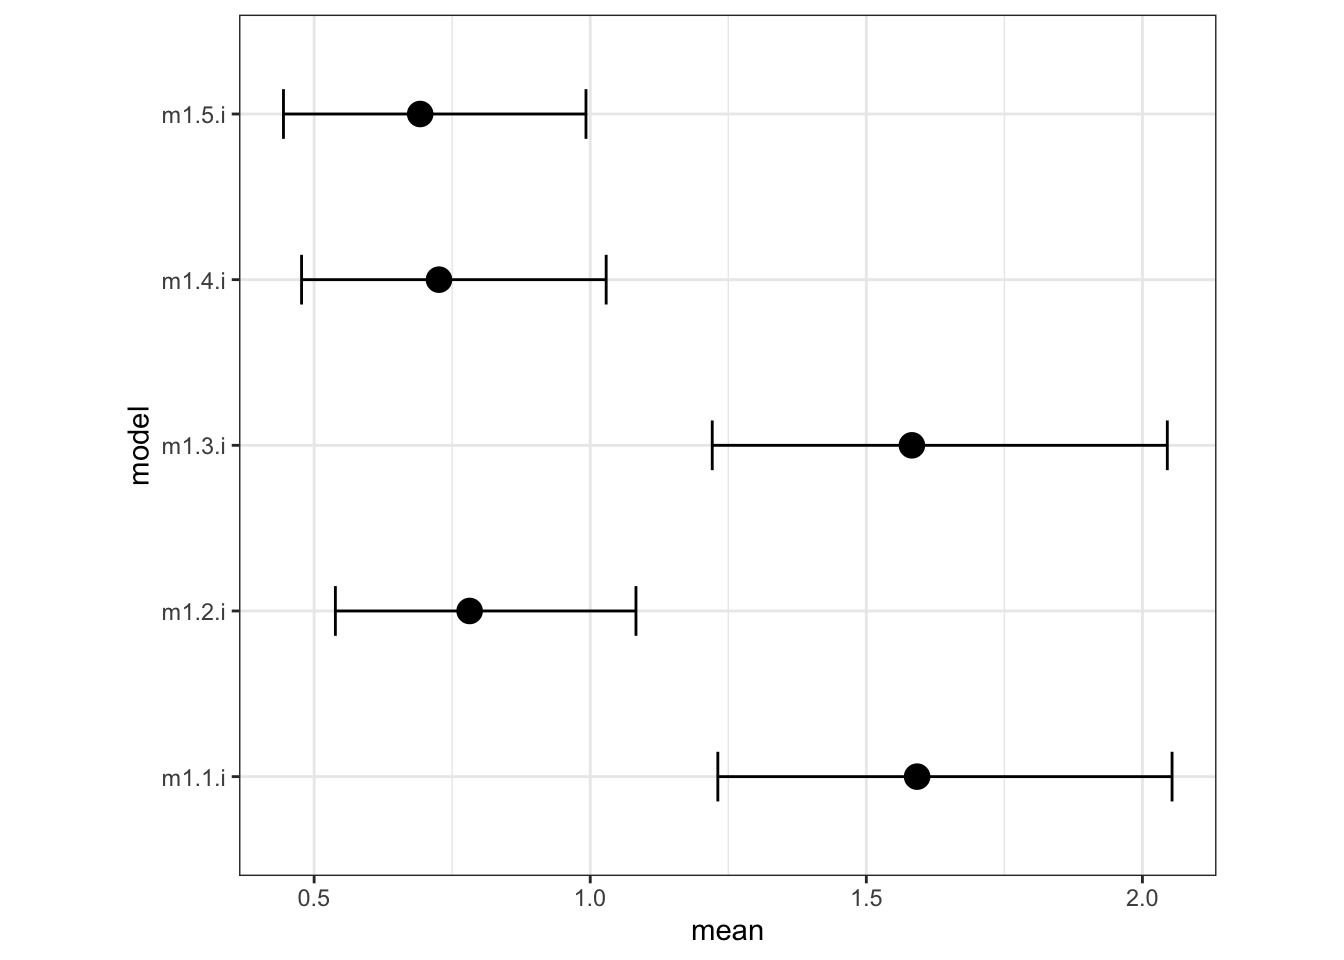
\includegraphics{rethinkingINLA_HW8_files/figure-latex/sigma.8.1 plot-1.pdf}

\hypertarget{section-1}{%
\section{2.}\label{section-1}}

\textbf{In 1980, a typical Bengali woman could have 5 or more children
in her lifetime. By the year 2000, a typical Bengali woman had only 2 or
3. You're going to look at a historical set of data, when contraception
was widely available but many families chose not to use it. These data
reside in data(bangladesh) and come from the 1988 Bangladesh Fertility
Survey. Each row is one of 1934 women. There are six variables, but you
can focus on two of them for this practice problem:}

\textbf{(1) district: ID number of administrative district each woman
resided in}

\textbf{(2) use.contraception: An indicator (0/1) of whether the woman
was using contraception}

\textbf{Focus on predicting use.contraception, clustered by
district\_id. Fit both:}

\textbf{1) a traditional fixed-effects model that uses an index variable
for district}

\textbf{2) a multilevel model with varying intercepts for district.}

Plot the predicted proportions of women in each district using
contraception, for both the fixed-effects model and the varying-effects
model. That is, make a plot in which district ID is on the horizontal
axis and expected proportion using contraception is on the vertical.
Make one plot for each model, or layer them on the same plot, as you
prefer. How do the models disagree? Can you explain the pattern of
disagreement? In particular, can you explain the most extreme cases of
disagreement, both why they happen where they do and why the models
reach different inferences?**

\begin{Shaded}
\begin{Highlighting}[]
\KeywordTok{library}\NormalTok{(rethinking)}
\KeywordTok{data}\NormalTok{(bangladesh)}
\NormalTok{d <-}\StringTok{ }\NormalTok{bangladesh}
\end{Highlighting}
\end{Shaded}

The first thing to do is ensure that the cluster variable, district, is
a contiguous set of integers. Recall that these values will be index
values inside the model. If there are gaps, you'll have parameters for
which there is no data to inform them. Worse, the model probably won't
run. Look at the unique values of the district variable:

\begin{Shaded}
\begin{Highlighting}[]
\KeywordTok{sort}\NormalTok{(}\KeywordTok{unique}\NormalTok{(d}\OperatorTok{$}\NormalTok{district))}
\end{Highlighting}
\end{Shaded}

\begin{verbatim}
##  [1]  1  2  3  4  5  6  7  8  9 10 11 12 13 14 15 16 17 18 19 20 21 22 23 24 25 26 27 28 29 30 31 32 33 34 35 36 37 38 39 40 41 42 43 44 45 46 47
## [48] 48 49 50 51 52 53 55 56 57 58 59 60 61
\end{verbatim}

District 54 is absent. So district isn't yet a good index variable,
because it's not contiguous. This is easy to fix. Just make a new
variable that is contiguous. This is enough to do it:

\begin{Shaded}
\begin{Highlighting}[]
\NormalTok{d}\OperatorTok{$}\NormalTok{district_id <-}\StringTok{ }\KeywordTok{as.integer}\NormalTok{(}\KeywordTok{as.factor}\NormalTok{(d}\OperatorTok{$}\NormalTok{district)) }
\KeywordTok{sort}\NormalTok{(}\KeywordTok{unique}\NormalTok{(d}\OperatorTok{$}\NormalTok{district_id))}
\end{Highlighting}
\end{Shaded}

\begin{verbatim}
##  [1]  1  2  3  4  5  6  7  8  9 10 11 12 13 14 15 16 17 18 19 20 21 22 23 24 25 26 27 28 29 30 31 32 33 34 35 36 37 38 39 40 41 42 43 44 45 46 47
## [48] 48 49 50 51 52 53 54 55 56 57 58 59 60
\end{verbatim}

Now there are 60 values, contiguous integers 1 to 60.

\hypertarget{traditional-fixed-effects-model-that-uses-an-index-variable-for-district}{%
\subsection{2.1 traditional fixed-effects model that uses an index
variable for
district}\label{traditional-fixed-effects-model-that-uses-an-index-variable-for-district}}

\hypertarget{rethinking-5}{%
\subsubsection{2.1 rethinking}\label{rethinking-5}}

\begin{Shaded}
\begin{Highlighting}[]
\NormalTok{dat_list <-}\StringTok{ }\KeywordTok{list}\NormalTok{(}
\DataTypeTok{C =}\NormalTok{ d}\OperatorTok{$}\NormalTok{use.contraception, }
\DataTypeTok{did =}\NormalTok{ d}\OperatorTok{$}\NormalTok{district_id}
\NormalTok{)}

\NormalTok{m2}\FloatTok{.1}\NormalTok{ <-}\StringTok{ }\KeywordTok{ulam}\NormalTok{( }\KeywordTok{alist}\NormalTok{(}
\NormalTok{C }\OperatorTok{~}\StringTok{ }\KeywordTok{bernoulli}\NormalTok{( p ),}
\KeywordTok{logit}\NormalTok{(p) <-}\StringTok{ }\NormalTok{a[did],}
\NormalTok{a[did] }\OperatorTok{~}\StringTok{ }\KeywordTok{normal}\NormalTok{( }\DecValTok{0}\NormalTok{ , }\FloatTok{1.5}\NormalTok{ )}
\NormalTok{) , }\DataTypeTok{data=}\NormalTok{dat_list , }\DataTypeTok{chains=}\DecValTok{4}\NormalTok{ , }\DataTypeTok{cores=}\DecValTok{4}\NormalTok{ , }\DataTypeTok{log_lik=}\OtherTok{TRUE}\NormalTok{ )}

\KeywordTok{precis}\NormalTok{(m2}\FloatTok{.1}\NormalTok{, }\DataTypeTok{depth =} \DecValTok{2}\NormalTok{)}
\end{Highlighting}
\end{Shaded}

\begin{verbatim}
##               mean        sd       5.5%       94.5%    n_eff     Rhat4
## a[1]  -1.047660116 0.2095908 -1.3816987 -0.71739447 4703.687 0.9984432
## a[2]  -0.596402631 0.4674239 -1.3434995  0.13003273 3260.155 0.9985068
## a[3]   1.241811792 1.1219090 -0.5256206  3.08744441 3026.802 0.9989061
## a[4]  -0.011083069 0.3648425 -0.5997161  0.56390235 4224.116 0.9986026
## a[5]  -0.566810128 0.3272602 -1.0901083 -0.04957457 3383.827 0.9985689
## a[6]  -0.873633655 0.2700627 -1.3151842 -0.44925598 4734.902 0.9995801
## a[7]  -0.893434425 0.4827446 -1.6916532 -0.13771922 4018.538 0.9983848
## a[8]  -0.484964742 0.3468814 -1.0480201  0.04757000 4311.207 0.9997675
## a[9]  -0.799574252 0.4324633 -1.5140264 -0.12618566 3466.509 0.9992037
## a[10] -1.983710355 0.7226824 -3.2078448 -0.88253861 2709.336 1.0002030
## a[11] -2.953258300 0.8270442 -4.4133831 -1.76842089 3397.298 0.9999033
## a[12] -0.610801613 0.4119704 -1.2630895  0.02381099 5153.156 0.9995279
## a[13] -0.328436107 0.4142077 -1.0178339  0.30286928 3968.230 0.9996938
## a[14]  0.514795871 0.1837075  0.2131496  0.80717058 3522.144 0.9987900
## a[15] -0.537210765 0.4268109 -1.2357433  0.12513458 5426.615 0.9985152
## a[16]  0.195809957 0.4326137 -0.4547552  0.85929818 4400.432 0.9988386
## a[17] -0.856921980 0.4268658 -1.5497628 -0.19273200 3628.908 0.9985756
## a[18] -0.649237541 0.3133901 -1.1601180 -0.14690795 4946.203 0.9984675
## a[19] -0.453343654 0.3921218 -1.0980582  0.18508872 4426.498 0.9989744
## a[20] -0.377068820 0.5116964 -1.2031215  0.41595580 5539.954 0.9984739
## a[21] -0.423586734 0.4736066 -1.1780628  0.29537565 5019.411 0.9985789
## a[22] -1.295370229 0.5192293 -2.1527558 -0.51209983 4117.695 0.9982467
## a[23] -0.944139074 0.5770646 -1.9053741 -0.05545977 5120.205 0.9985345
## a[24] -2.025318983 0.7322664 -3.2648327 -0.94104669 4331.403 0.9991579
## a[25] -0.212968205 0.2461773 -0.6059332  0.17461144 3311.187 0.9991349
## a[26] -0.424927697 0.5338276 -1.2935595  0.44239886 4660.719 0.9988737
## a[27] -1.442316610 0.3540959 -2.0339859 -0.89830564 3522.921 0.9991765
## a[28] -1.099159300 0.3351535 -1.6612863 -0.58444179 5660.933 0.9986875
## a[29] -0.901370808 0.3817938 -1.5112410 -0.30120180 4382.463 0.9989887
## a[30] -0.035894010 0.2509450 -0.4332923  0.37187869 4304.807 0.9988399
## a[31] -0.178674363 0.3510672 -0.7425508  0.37786113 4403.994 0.9985657
## a[32] -1.271058095 0.4707135 -2.0557610 -0.53497091 3440.314 0.9994473
## a[33] -0.276621042 0.5354301 -1.1333498  0.59677763 4087.705 0.9986470
## a[34]  0.626883438 0.3342194  0.1023593  1.17718994 3580.220 0.9985276
## a[35]  0.002177843 0.2798970 -0.4539693  0.44921583 4768.152 0.9986057
## a[36] -0.567202784 0.4809086 -1.3365697  0.17765172 5181.891 0.9987672
## a[37]  0.152445979 0.5325720 -0.7217905  0.98814393 3362.410 1.0000426
## a[38] -0.837403781 0.5245372 -1.7144144  0.00279963 4178.406 0.9984092
## a[39]  0.003214860 0.3721672 -0.5955309  0.60358341 4957.121 0.9986155
## a[40] -0.144017244 0.3166898 -0.6556812  0.35402117 4269.042 0.9989453
## a[41] -0.009197519 0.3844950 -0.6221775  0.60118022 3512.845 0.9993219
## a[42]  0.170126346 0.5787394 -0.7245689  1.07152381 4264.511 0.9987139
## a[43]  0.135679875 0.2811021 -0.3176799  0.57051058 3489.240 0.9989356
## a[44] -1.188541003 0.4178192 -1.8682347 -0.54217937 3860.169 0.9986436
## a[45] -0.676605647 0.3405241 -1.2257012 -0.14230439 3662.538 1.0001672
## a[46]  0.090573020 0.2176561 -0.2644962  0.43929096 4851.991 0.9985974
## a[47] -0.127922898 0.5208258 -0.9785667  0.68951733 4221.132 0.9989432
## a[48]  0.089979766 0.3075047 -0.4157302  0.59387411 4412.335 0.9995868
## a[49] -1.739901964 1.0346414 -3.4464706 -0.14314954 3717.925 0.9992835
## a[50] -0.099699980 0.4448886 -0.7951214  0.59940475 3896.657 0.9986767
## a[51] -0.149923811 0.3299442 -0.6708611  0.38214505 3505.561 1.0002054
## a[52] -0.220517882 0.2398554 -0.6029594  0.15150656 5234.284 0.9985499
## a[53] -0.296602853 0.4623373 -1.0481501  0.43782493 3404.776 0.9987314
## a[54] -1.224038872 0.8413025 -2.6185323  0.05889909 4500.993 0.9992736
## a[55]  0.301019439 0.2955932 -0.1616943  0.78419868 4525.593 0.9991510
## a[56] -1.390741604 0.4645985 -2.1715633 -0.67601733 3583.332 0.9983579
## a[57] -0.174149533 0.3499630 -0.7455571  0.37589799 4359.291 1.0001223
## a[58] -1.729711204 0.7624694 -2.9899310 -0.57992382 3789.217 0.9987956
## a[59] -1.214428837 0.4046465 -1.8716364 -0.55666550 4919.099 0.9992347
## a[60] -1.268323809 0.3755206 -1.8818992 -0.69391120 3829.616 0.9983795
\end{verbatim}

\hypertarget{inla-5}{%
\subsubsection{2.1 inla}\label{inla-5}}

\begin{Shaded}
\begin{Highlighting}[]
\KeywordTok{library}\NormalTok{(brinla)}
\KeywordTok{library}\NormalTok{(INLA)}
\KeywordTok{library}\NormalTok{(tidyverse)}

\NormalTok{d2.i <-}\StringTok{ }\NormalTok{d }\OperatorTok\StringTok{ }
\StringTok{  }\KeywordTok{mutate}\NormalTok{(}\DataTypeTok{did=} \KeywordTok{paste}\NormalTok{(}\StringTok{"d"}\NormalTok{, }\KeywordTok{as.integer}\NormalTok{(d}\OperatorTok{$}\NormalTok{district_id), }\DataTypeTok{sep=} \StringTok{"."}\NormalTok{), }
         \DataTypeTok{d.value=} \DecValTok{1}
\NormalTok{         ) }\OperatorTok\StringTok{ }
\StringTok{  }\KeywordTok{spread}\NormalTok{(did, d.value)}

\CommentTok{#use this to quickly make a list of the index vbles to include in the model }
\NormalTok{did_formula <-}\StringTok{ }\KeywordTok{paste}\NormalTok{(}\StringTok{"d"}\NormalTok{, }\DecValTok{1}\OperatorTok{:}\DecValTok{60}\NormalTok{, }\DataTypeTok{sep=}\StringTok{"."}\NormalTok{, }\DataTypeTok{collapse =} \StringTok{"+"}\NormalTok{)}


\NormalTok{m2.}\FloatTok{1.}\NormalTok{i <-}\StringTok{ }\KeywordTok{inla}\NormalTok{(use.contraception }\OperatorTok{~}\StringTok{ }\NormalTok{d}\FloatTok{.1}\OperatorTok{+}\NormalTok{d}\FloatTok{.2}\OperatorTok{+}\NormalTok{d}\FloatTok{.3}\OperatorTok{+}\NormalTok{d}\FloatTok{.4}\OperatorTok{+}\NormalTok{d}\FloatTok{.5}\OperatorTok{+}\NormalTok{d}\FloatTok{.6}\OperatorTok{+}\NormalTok{d}\FloatTok{.7}\OperatorTok{+}\NormalTok{d}\FloatTok{.8}\OperatorTok{+}\NormalTok{d}\FloatTok{.9}\OperatorTok{+}\NormalTok{d}\FloatTok{.10}\OperatorTok{+}\NormalTok{d}\FloatTok{.11}\OperatorTok{+}\NormalTok{d}\FloatTok{.12}\OperatorTok{+}\NormalTok{d}\FloatTok{.13}\OperatorTok{+}\NormalTok{d}\FloatTok{.14}\OperatorTok{+}\NormalTok{d}\FloatTok{.15}\OperatorTok{+}\NormalTok{d}\FloatTok{.16}\OperatorTok{+}\NormalTok{d}\FloatTok{.17}\OperatorTok{+}\NormalTok{d}\FloatTok{.18}\OperatorTok{+}\NormalTok{d}\FloatTok{.19}\OperatorTok{+}\NormalTok{d}\FloatTok{.20}\OperatorTok{+}\NormalTok{d}\FloatTok{.21}\OperatorTok{+}\NormalTok{d}\FloatTok{.22}\OperatorTok{+}\NormalTok{d}\FloatTok{.23}\OperatorTok{+}\NormalTok{d}\FloatTok{.24}\OperatorTok{+}\NormalTok{d}\FloatTok{.25}\OperatorTok{+}\NormalTok{d}\FloatTok{.26}\OperatorTok{+}\NormalTok{d}\FloatTok{.27}\OperatorTok{+}\NormalTok{d}\FloatTok{.28}\OperatorTok{+}\NormalTok{d}\FloatTok{.29}\OperatorTok{+}\NormalTok{d}\FloatTok{.30}\OperatorTok{+}\NormalTok{d}\FloatTok{.31}\OperatorTok{+}\NormalTok{d}\FloatTok{.32}\OperatorTok{+}\NormalTok{d}\FloatTok{.33}\OperatorTok{+}\NormalTok{d}\FloatTok{.34}\OperatorTok{+}\NormalTok{d}\FloatTok{.35}\OperatorTok{+}\NormalTok{d}\FloatTok{.36}\OperatorTok{+}\NormalTok{d}\FloatTok{.37}\OperatorTok{+}\NormalTok{d}\FloatTok{.38}\OperatorTok{+}\NormalTok{d}\FloatTok{.39}\OperatorTok{+}\NormalTok{d}\FloatTok{.40}\OperatorTok{+}\NormalTok{d}\FloatTok{.41}\OperatorTok{+}\NormalTok{d}\FloatTok{.42}\OperatorTok{+}\NormalTok{d}\FloatTok{.43}\OperatorTok{+}\NormalTok{d}\FloatTok{.44}\OperatorTok{+}\NormalTok{d}\FloatTok{.45}\OperatorTok{+}\NormalTok{d}\FloatTok{.46}\OperatorTok{+}\NormalTok{d}\FloatTok{.47}\OperatorTok{+}\NormalTok{d}\FloatTok{.48}\OperatorTok{+}\NormalTok{d}\FloatTok{.49}\OperatorTok{+}\NormalTok{d}\FloatTok{.50}\OperatorTok{+}\NormalTok{d}\FloatTok{.51}\OperatorTok{+}\NormalTok{d}\FloatTok{.52}\OperatorTok{+}\NormalTok{d}\FloatTok{.53}\OperatorTok{+}\NormalTok{d}\FloatTok{.54}\OperatorTok{+}\NormalTok{d}\FloatTok{.55}\OperatorTok{+}\NormalTok{d}\FloatTok{.56}\OperatorTok{+}\NormalTok{d}\FloatTok{.57}\OperatorTok{+}\NormalTok{d}\FloatTok{.58}\OperatorTok{+}\NormalTok{d}\FloatTok{.59}\OperatorTok{+}\NormalTok{d}\FloatTok{.60}\NormalTok{, }\DataTypeTok{data=}\NormalTok{ d2.i, }\DataTypeTok{family =} \StringTok{"binomial"}\NormalTok{, }
              \DataTypeTok{Ntrials =} \DecValTok{1}\NormalTok{, }\CommentTok{#Ntrials = 1 for bernoulli}
              \DataTypeTok{control.family =} \KeywordTok{list}\NormalTok{(}\DataTypeTok{control.link=}\KeywordTok{list}\NormalTok{(}\DataTypeTok{model=}\StringTok{"logit"}\NormalTok{)),}
              \DataTypeTok{control.fixed =} \KeywordTok{list}\NormalTok{(}
        \DataTypeTok{mean=}  \DecValTok{0}\NormalTok{ ,}
        \DataTypeTok{prec=} \DecValTok{1}\OperatorTok{/}\NormalTok{(}\FloatTok{1.5}\OperatorTok{^}\DecValTok{2}\NormalTok{)),}
              \DataTypeTok{control.predictor=}\KeywordTok{list}\NormalTok{(}\DataTypeTok{link=}\DecValTok{1}\NormalTok{, }\DataTypeTok{compute=}\NormalTok{T),}
              \DataTypeTok{control.compute=}\KeywordTok{list}\NormalTok{(}\DataTypeTok{config=}\NormalTok{T, }\DataTypeTok{waic=} \OtherTok{TRUE}\NormalTok{))}
\KeywordTok{summary}\NormalTok{(m2.}\FloatTok{1.}\NormalTok{i)}
\end{Highlighting}
\end{Shaded}

\begin{verbatim}
## 
## Call:
##    c("inla(formula = use.contraception ~ d.1 + d.2 + d.3 + d.4 + d.5 + ", " d.6 + d.7 + d.8 + d.9 + d.10 + d.11 + d.12 + d.13 + d.14 
##    + ", " d.15 + d.16 + d.17 + d.18 + d.19 + d.20 + d.21 + d.22 + d.23 + ", " d.24 + d.25 + d.26 + d.27 + d.28 + d.29 + d.30 + d.31 + 
##    d.32 + ", " d.33 + d.34 + d.35 + d.36 + d.37 + d.38 + d.39 + d.40 + d.41 + ", " d.42 + d.43 + d.44 + d.45 + d.46 + d.47 + d.48 + 
##    d.49 + d.50 + ", " d.51 + d.52 + d.53 + d.54 + d.55 + d.56 + d.57 + d.58 + d.59 + ", " d.60, family = \"binomial\", data = d2.i, 
##    Ntrials = 1, control.compute = list(config = T, ", " waic = TRUE), control.predictor = list(link = 1, compute = T), ", " 
##    control.family = list(control.link = list(model = \"logit\")), ", " control.fixed = list(mean = 0, prec = 1/(1.5^2)))") 
## Time used:
##     Pre = 5, Running = 0.485, Post = 3.7, Total = 9.18 
## Fixed effects:
##               mean    sd 0.025quant 0.5quant 0.975quant   mode kld
## (Intercept) -0.634 0.204     -1.035   -0.634     -0.234 -0.634   0
## d.1         -0.427 0.290     -1.001   -0.425      0.136 -0.421   0
## d.2          0.009 0.484     -0.967    0.017      0.936  0.034   0
## d.3          1.421 1.074     -0.583    1.382      3.640  1.306   0
## d.4          0.599 0.404     -0.194    0.600      1.391  0.600   0
## d.5          0.048 0.380     -0.709    0.052      0.782  0.060   0
## d.6         -0.247 0.333     -0.911   -0.244      0.397 -0.237   0
## d.7         -0.294 0.525     -1.367   -0.279      0.695 -0.250   0
## d.8          0.128 0.384     -0.636    0.131      0.871  0.138   0
## d.9         -0.183 0.471     -1.136   -0.173      0.713 -0.153   0
## d.10        -1.349 0.750     -2.950   -1.302     -0.002 -1.208   0
## d.11        -2.343 0.845     -4.166   -2.281     -0.851 -2.155   0
## d.12        -0.012 0.424     -0.861   -0.006      0.803  0.006   0
## d.13         0.274 0.443     -0.606    0.278      1.132  0.286   0
## d.14         1.138 0.276      0.599    1.137      1.681  1.136   0
## d.15         0.064 0.465     -0.869    0.071      0.957  0.085   0
## d.16         0.767 0.469     -0.148    0.766      1.692  0.762   0
## d.17        -0.239 0.467     -1.187   -0.229      0.649 -0.208   0
## d.18        -0.030 0.360     -0.747   -0.027      0.666 -0.019   0
## d.19         0.150 0.434     -0.716    0.155      0.987  0.165   0
## d.20         0.200 0.530     -0.863    0.208      1.220  0.223   0
## d.21         0.161 0.497     -0.834    0.168      1.117  0.182   0
## d.22        -0.673 0.542     -1.796   -0.652      0.332 -0.611   0
## d.23        -0.337 0.566     -1.501   -0.318      0.724 -0.282   0
## d.24        -1.413 0.743     -3.001   -1.367     -0.079 -1.272   0
## d.25         0.413 0.314     -0.205    0.413      1.027  0.415   0
## d.26         0.139 0.563     -0.994    0.149      1.216  0.169   0
## d.27        -0.826 0.418     -1.679   -0.814     -0.037 -0.791   0
## d.28        -0.476 0.377     -1.235   -0.470      0.244 -0.456   0
## d.29        -0.291 0.424     -1.148   -0.283      0.517 -0.266   0
## d.30         0.585 0.321     -0.046    0.585      1.214  0.585   0
## d.31         0.428 0.392     -0.347    0.429      1.193  0.432   0
## d.32        -0.641 0.502     -1.676   -0.624      0.296 -0.590   0
## d.33         0.304 0.541     -0.775    0.310      1.348  0.322   0
## d.34         1.222 0.394      0.461    1.217      2.008  1.208   0
## d.35         0.612 0.345     -0.066    0.612      1.289  0.612   0
## d.36         0.020 0.514     -1.018    0.030      1.002  0.049   0
## d.37         0.693 0.551     -0.384    0.692      1.777  0.690   0
## d.38        -0.252 0.574     -1.428   -0.235      0.825 -0.200   0
## d.39         0.594 0.425     -0.241    0.595      1.427  0.595   0
## d.40         0.467 0.364     -0.251    0.468      1.178  0.470   0
## d.41         0.594 0.425     -0.241    0.595      1.427  0.595   0
## d.42         0.703 0.587     -0.445    0.701      1.859  0.698   0
## d.43         0.739 0.353      0.048    0.739      1.433  0.737   0
## d.44        -0.575 0.474     -1.546   -0.561      0.316 -0.532   0
## d.45        -0.061 0.384     -0.828   -0.056      0.680 -0.047   0
## d.46         0.713 0.293      0.139    0.713      1.288  0.712   0
## d.47         0.447 0.523     -0.590    0.450      1.464  0.456   0
## d.48         0.700 0.360     -0.006    0.700      1.408  0.699   0
## d.49        -1.230 1.047     -3.465   -1.166      0.651 -1.035   0
## d.50         0.483 0.478     -0.461    0.485      1.415  0.489   0
## d.51         0.449 0.377     -0.294    0.451      1.185  0.453   0
## d.52         0.391 0.323     -0.244    0.392      1.022  0.394   0
## d.53         0.286 0.482     -0.675    0.290      1.219  0.300   0
## d.54        -0.669 0.837     -2.437   -0.625      0.856 -0.537   0
## d.55         0.913 0.355      0.221    0.912      1.613  0.909   0
## d.56        -0.777 0.495     -1.799   -0.759      0.144 -0.724   0
## d.57         0.428 0.392     -0.347    0.429      1.193  0.432   0
## d.58        -1.120 0.776     -2.772   -1.074      0.278 -0.980   0
## d.59        -0.601 0.448     -1.514   -0.588      0.243 -0.563   0
## d.60        -0.635 0.409     -1.465   -0.625      0.140 -0.606   0
## 
## Expected number of effective parameters(stdev): 54.05(0.00)
## Number of equivalent replicates : 35.78 
## 
## Watanabe-Akaike information criterion (WAIC) ...: 2521.28
## Effective number of parameters .................: 52.54
## 
## Marginal log-Likelihood:  -1291.66 
## Posterior marginals for the linear predictor and
##  the fitted values are computed
\end{verbatim}

\hypertarget{varying-intercepts-model-1}{%
\subsection{2.2 varying intercepts
model}\label{varying-intercepts-model-1}}

\hypertarget{rethinking-6}{%
\subsubsection{2.2 rethinking}\label{rethinking-6}}

\begin{Shaded}
\begin{Highlighting}[]
\NormalTok{m2}\FloatTok{.2}\NormalTok{ <-}\StringTok{ }\KeywordTok{ulam}\NormalTok{( }\KeywordTok{alist}\NormalTok{(}
\NormalTok{C }\OperatorTok{~}\StringTok{ }\KeywordTok{bernoulli}\NormalTok{( p ),}
\KeywordTok{logit}\NormalTok{(p) <-}\StringTok{ }\NormalTok{a[did],}
\NormalTok{a[did] }\OperatorTok{~}\StringTok{ }\KeywordTok{normal}\NormalTok{( a_bar , sigma ),}
\NormalTok{a_bar }\OperatorTok{~}\StringTok{ }\KeywordTok{normal}\NormalTok{( }\DecValTok{0}\NormalTok{ , }\FloatTok{1.5}\NormalTok{ ),}
\NormalTok{sigma }\OperatorTok{~}\StringTok{ }\KeywordTok{exponential}\NormalTok{( }\DecValTok{1}\NormalTok{ )}
\NormalTok{) ,}\DataTypeTok{data=}\NormalTok{dat_list , }\DataTypeTok{chains=}\DecValTok{4}\NormalTok{ , }\DataTypeTok{cores=}\DecValTok{4}\NormalTok{ , }\DataTypeTok{log_lik=}\OtherTok{TRUE}\NormalTok{ )}

\KeywordTok{precis}\NormalTok{(m2}\FloatTok{.2}\NormalTok{, }\DataTypeTok{depth=} \DecValTok{2}\NormalTok{)}
\end{Highlighting}
\end{Shaded}

\begin{verbatim}
##               mean         sd       5.5%        94.5%     n_eff     Rhat4
## a[1]  -0.992576303 0.19377086 -1.3138594 -0.691778504 2785.7617 1.0009880
## a[2]  -0.593394247 0.35651291 -1.1575224 -0.025804366 2606.7649 0.9982014
## a[3]  -0.231519703 0.47772294 -0.9435780  0.563448693 2900.4680 0.9987246
## a[4]  -0.188480633 0.29175618 -0.6528299  0.273372403 3245.4322 0.9992062
## a[5]  -0.571490831 0.28629961 -1.0250540 -0.127105622 2810.6188 1.0001870
## a[6]  -0.810222394 0.24685867 -1.2053243 -0.428673558 2835.6122 0.9997776
## a[7]  -0.748343070 0.35357731 -1.3192644 -0.214360252 2864.8223 0.9984335
## a[8]  -0.516782598 0.29451072 -0.9796936 -0.043706869 3974.8547 0.9996529
## a[9]  -0.710828746 0.33759227 -1.2685853 -0.187166314 2878.0506 1.0003681
## a[10] -1.130063737 0.41699783 -1.8164682 -0.494361243 2236.0475 0.9990703
## a[11] -1.540054094 0.42635361 -2.2267722 -0.891144497 1343.2481 1.0015071
## a[12] -0.613740919 0.31708758 -1.1390898 -0.110689673 3403.6909 0.9985627
## a[13] -0.420429220 0.32612394 -0.9375511  0.092487415 2767.6195 0.9989454
## a[14]  0.391144100 0.18309369  0.1072187  0.683638042 2712.7572 0.9991113
## a[15] -0.558561902 0.33615036 -1.0877087 -0.037774761 4123.5710 0.9983679
## a[16] -0.130130707 0.34201302 -0.6641128  0.452982978 3954.0179 0.9985978
## a[17] -0.752083961 0.33995891 -1.3284303 -0.230680695 3021.9946 1.0000496
## a[18] -0.642047026 0.26036271 -1.0534557 -0.234917962 3246.9353 0.9986047
## a[19] -0.499375344 0.32291593 -1.0073947 -0.005192187 3636.8338 0.9984635
## a[20] -0.493824570 0.37568359 -1.0799898  0.117927311 3381.6217 0.9985119
## a[21] -0.499767149 0.36590856 -1.0660328  0.065247205 3528.0586 0.9997141
## a[22] -0.963752045 0.37345047 -1.5663655 -0.397717027 2919.7282 0.9989256
## a[23] -0.755837894 0.37074316 -1.3680409 -0.166292488 3103.4418 0.9987398
## a[24] -1.176035196 0.42050479 -1.8756030 -0.545891296 1460.7124 0.9991237
## a[25] -0.282665473 0.22679241 -0.6424053  0.071821168 4074.3117 0.9990370
## a[26] -0.520571546 0.39258635 -1.1439735  0.094486881 3598.8769 0.9989668
## a[27] -1.175913842 0.30122602 -1.6632214 -0.708747431 3298.7436 0.9991740
## a[28] -0.966309770 0.28097025 -1.4170199 -0.512432620 3039.2377 0.9989804
## a[29] -0.799835579 0.32093238 -1.3060814 -0.274703460 2826.0271 0.9989692
## a[30] -0.143208774 0.22699045 -0.5003997  0.224913639 4372.4204 0.9994127
## a[31] -0.303901793 0.29704836 -0.7946707  0.163868891 3370.1822 1.0006201
## a[32] -0.973036861 0.35340061 -1.5677258 -0.441036725 2466.5111 0.9993772
## a[33] -0.424600248 0.38954718 -1.0642620  0.218171853 3874.8011 0.9999891
## a[34]  0.279040943 0.29350334 -0.1648151  0.756194728 2856.4671 0.9988745
## a[35] -0.139369718 0.24502977 -0.5311149  0.259537514 3448.1295 0.9986007
## a[36] -0.572542774 0.37517312 -1.1674523 -0.014222490 4377.7505 0.9992506
## a[37] -0.220214308 0.37913654 -0.8343030  0.395140351 3052.1607 0.9996100
## a[38] -0.706924631 0.36885788 -1.3076656 -0.131569364 2765.4270 0.9995794
## a[39] -0.206035757 0.33419959 -0.7314593  0.319146450 4084.3704 0.9984645
## a[40] -0.260407422 0.26744104 -0.6944026  0.160920340 3104.9571 0.9985270
## a[41] -0.209790889 0.30926106 -0.7039166  0.290240731 4184.9112 0.9989893
## a[42] -0.228457194 0.40360603 -0.8801795  0.434961403 3376.2192 0.9996645
## a[43] -0.038461675 0.26424276 -0.4615295  0.381500885 3342.9985 0.9989571
## a[44] -0.959753393 0.33201993 -1.4941089 -0.426011158 3065.3730 0.9986545
## a[45] -0.659027869 0.28130598 -1.1065427 -0.210275110 3321.5766 0.9989456
## a[46] -0.007147924 0.20538768 -0.3340400  0.314759934 3225.1956 0.9989689
## a[47] -0.333402316 0.35415750 -0.8741818  0.226521916 2895.9662 0.9996403
## a[48] -0.080057495 0.26984620 -0.5167205  0.347119384 2968.2032 0.9987146
## a[49] -0.840680577 0.44599705 -1.5530859 -0.146792274 1995.0294 0.9998875
## a[50] -0.313103629 0.33916906 -0.8399939  0.256986053 3261.1808 0.9996062
## a[51] -0.274203332 0.27338106 -0.7186504  0.150663625 3524.6563 0.9985691
## a[52] -0.298821900 0.22710069 -0.6635522  0.061712742 3705.8757 1.0013545
## a[53] -0.428169152 0.35247433 -0.9984944  0.150463290 3402.5717 0.9989971
## a[54] -0.786316839 0.45402287 -1.5287677 -0.096797840 2015.0305 0.9994580
## a[55]  0.094178770 0.25809061 -0.3126327  0.510629247 2650.0100 0.9986666
## a[56] -1.061666397 0.34392922 -1.6441917 -0.529947246 2342.7367 0.9992427
## a[57] -0.296532110 0.29869526 -0.7686459  0.182014937 3889.0160 0.9990523
## a[58] -1.001688012 0.43067942 -1.6913387 -0.356425952 2049.9861 0.9995093
## a[59] -0.984409828 0.31542264 -1.4804884 -0.495681906 3146.0027 0.9990056
## a[60] -1.054868930 0.29388513 -1.5362391 -0.583270515 2379.6651 0.9990559
## a_bar -0.539149824 0.08540223 -0.6794501 -0.405158579 1564.2535 1.0003799
## sigma  0.512779330 0.08209941  0.3913976  0.651629007  599.4438 1.0016994
\end{verbatim}

\hypertarget{inla-6}{%
\subsubsection{2.2 inla}\label{inla-6}}

\begin{Shaded}
\begin{Highlighting}[]
\NormalTok{m2.}\FloatTok{2.}\NormalTok{i <-}\StringTok{ }\KeywordTok{inla}\NormalTok{(use.contraception }\OperatorTok{~}\StringTok{ }\KeywordTok{f}\NormalTok{(district_id, }\DataTypeTok{model=}\StringTok{"iid"}\NormalTok{), }\DataTypeTok{data=}\NormalTok{ d2.i, }\DataTypeTok{family =} \StringTok{"binomial"}\NormalTok{, }
              \DataTypeTok{Ntrials =} \DecValTok{1}\NormalTok{, }\CommentTok{#Ntrials = 1 for bernoulli}
              \DataTypeTok{control.family =} \KeywordTok{list}\NormalTok{(}\DataTypeTok{control.link=}\KeywordTok{list}\NormalTok{(}\DataTypeTok{model=}\StringTok{"logit"}\NormalTok{)),}
              \DataTypeTok{control.fixed =} \KeywordTok{list}\NormalTok{(}
        \DataTypeTok{mean.intercept=}  \DecValTok{0}\NormalTok{ ,}
        \DataTypeTok{prec.intercept=} \DecValTok{1}\OperatorTok{/}\NormalTok{(}\FloatTok{1.5}\OperatorTok{^}\DecValTok{2}\NormalTok{)),}
              \DataTypeTok{control.predictor=}\KeywordTok{list}\NormalTok{(}\DataTypeTok{link=}\DecValTok{1}\NormalTok{, }\DataTypeTok{compute=}\NormalTok{T),}
              \DataTypeTok{control.compute=}\KeywordTok{list}\NormalTok{(}\DataTypeTok{config=}\NormalTok{T, }\DataTypeTok{waic=} \OtherTok{TRUE}\NormalTok{))}
\KeywordTok{summary}\NormalTok{(m2.}\FloatTok{2.}\NormalTok{i)}
\end{Highlighting}
\end{Shaded}

\begin{verbatim}
## 
## Call:
##    c("inla(formula = use.contraception ~ f(district_id, model = \"iid\"), ", " family = \"binomial\", data = d2.i, Ntrials = 1, 
##    control.compute = list(config = T, ", " waic = TRUE), control.predictor = list(link = 1, compute = T), ", " control.family = 
##    list(control.link = list(model = \"logit\")), ", " control.fixed = list(mean.intercept = 0, prec.intercept = 1/(1.5^2)))" ) 
## Time used:
##     Pre = 3.44, Running = 8.72, Post = 0.6, Total = 12.8 
## Fixed effects:
##               mean    sd 0.025quant 0.5quant 0.975quant   mode kld
## (Intercept) -0.532 0.084     -0.701   -0.531     -0.371 -0.528   0
## 
## Random effects:
##   Name     Model
##     district_id IID model
## 
## Model hyperparameters:
##                           mean   sd 0.025quant 0.5quant 0.975quant mode
## Precision for district_id 4.72 1.64       2.38     4.43       8.72 3.95
## 
## Expected number of effective parameters(stdev): 33.99(4.22)
## Number of equivalent replicates : 56.89 
## 
## Watanabe-Akaike information criterion (WAIC) ...: 2514.73
## Effective number of parameters .................: 33.32
## 
## Marginal log-Likelihood:  -1278.85 
## Posterior marginals for the linear predictor and
##  the fitted values are computed
\end{verbatim}

\begin{Shaded}
\begin{Highlighting}[]
\KeywordTok{bri.hyperpar.summary}\NormalTok{(m2.}\FloatTok{2.}\NormalTok{i)}
\end{Highlighting}
\end{Shaded}

\begin{verbatim}
##                         mean         sd    q0.025      q0.5    q0.975      mode
## SD for district_id 0.4799266 0.07896511 0.3386587 0.4748979 0.6490092 0.4657703
\end{verbatim}

Side note: this is how you calculate the sd from the hyperprior
(\(\sigma\))

\begin{Shaded}
\begin{Highlighting}[]
\KeywordTok{bri.hyperpar.summary}\NormalTok{(m2.}\FloatTok{2.}\NormalTok{i)}
\end{Highlighting}
\end{Shaded}

\begin{verbatim}
##                         mean         sd    q0.025      q0.5    q0.975      mode
## SD for district_id 0.4799266 0.07896511 0.3386587 0.4748979 0.6490092 0.4657703
\end{verbatim}

\begin{Shaded}
\begin{Highlighting}[]
\CommentTok{# hyperparameter of the precision}
\NormalTok{m2.}\FloatTok{2.}\NormalTok{i.prec <-}\StringTok{ }\NormalTok{m2.}\FloatTok{2.}\NormalTok{i}\OperatorTok{$}\NormalTok{internal.marginals.hyperpar}

\CommentTok{#transform precision to sd using inla.tmarginal}
\CommentTok{#m2.2.i.prec[[1]] is used to access the actual values inside the list}
\NormalTok{m2.}\FloatTok{2.}\NormalTok{i.sd <-}\StringTok{ }\KeywordTok{inla.tmarginal}\NormalTok{(}\ControlFlowTok{function}\NormalTok{(x) }\KeywordTok{sqrt}\NormalTok{(}\KeywordTok{exp}\NormalTok{(}\OperatorTok{-}\NormalTok{x)), m2.}\FloatTok{2.}\NormalTok{i.prec[[}\DecValTok{1}\NormalTok{]])}
\CommentTok{#plot the post of the sd per district (sigma)}
\KeywordTok{plot}\NormalTok{(m2.}\FloatTok{2.}\NormalTok{i.sd)}
\end{Highlighting}
\end{Shaded}

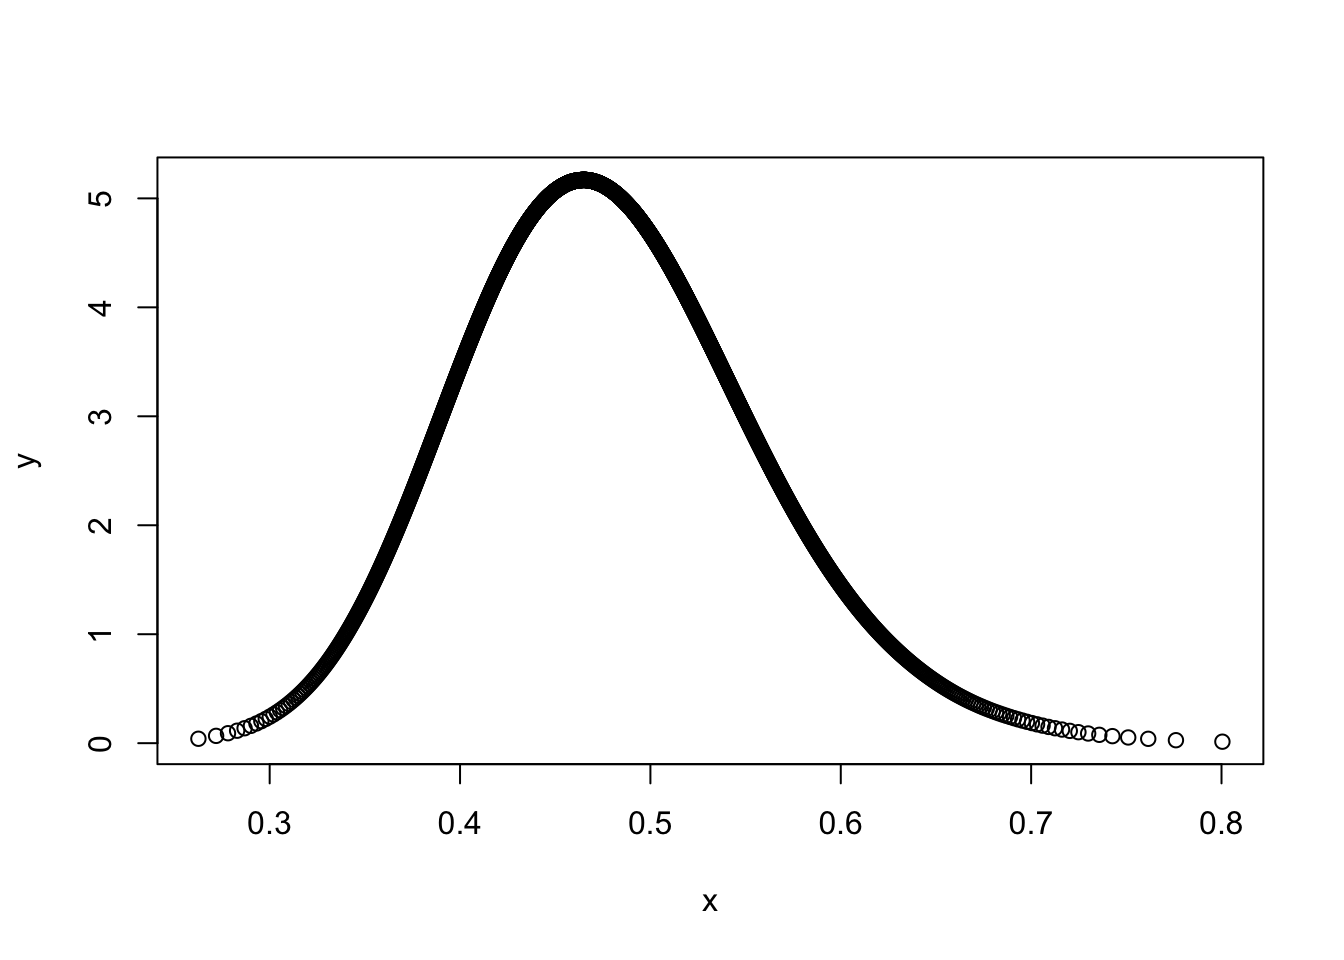
\includegraphics{rethinkingINLA_HW8_files/figure-latex/8.2.2 inla hyper sd-1.pdf}

\begin{Shaded}
\begin{Highlighting}[]
\CommentTok{#summary stats for the sd }
\NormalTok{m2.}\FloatTok{2.}\NormalTok{i.sd.sum <-}\StringTok{ }\KeywordTok{inla.zmarginal}\NormalTok{(m2.}\FloatTok{2.}\NormalTok{i.sd)}
\end{Highlighting}
\end{Shaded}

\begin{verbatim}
## Mean            0.479927 
## Stdev           0.0789651 
## Quantile  0.025 0.338659 
## Quantile  0.25  0.424454 
## Quantile  0.5   0.474898 
## Quantile  0.75  0.529795 
## Quantile  0.975 0.649009
\end{verbatim}

\begin{Shaded}
\begin{Highlighting}[]
\CommentTok{# this coincides perfectly with the result from bri.hyperpar.summary}
\end{Highlighting}
\end{Shaded}

\hypertarget{plot-of-posterior-mean-probabilities-in-each-district}{%
\subsection{2.3 plot of posterior mean probabilities in each
district}\label{plot-of-posterior-mean-probabilities-in-each-district}}

Now let's extract the samples, compute posterior mean probabilities in
each district, and plot it all:

\hypertarget{plot-rethinking}{%
\subsubsection{plot rethinking}\label{plot-rethinking}}

\begin{Shaded}
\begin{Highlighting}[]
\NormalTok{post1 <-}\StringTok{ }\KeywordTok{extract.samples}\NormalTok{( m2}\FloatTok{.1}\NormalTok{ ) }
\NormalTok{post2 <-}\StringTok{ }\KeywordTok{extract.samples}\NormalTok{( m2}\FloatTok{.2}\NormalTok{ )}
\NormalTok{p1 <-}\StringTok{ }\KeywordTok{apply}\NormalTok{( }\KeywordTok{inv_logit}\NormalTok{(post1}\OperatorTok{$}\NormalTok{a) , }\DecValTok{2}\NormalTok{ , mean ) }
\NormalTok{p2 <-}\StringTok{ }\KeywordTok{apply}\NormalTok{( }\KeywordTok{inv_logit}\NormalTok{(post2}\OperatorTok{$}\NormalTok{a) , }\DecValTok{2}\NormalTok{ , mean )}
\NormalTok{nd <-}\StringTok{ }\KeywordTok{max}\NormalTok{(dat_list}\OperatorTok{$}\NormalTok{did)}
\KeywordTok{plot}\NormalTok{( }\OtherTok{NULL}\NormalTok{ , }\DataTypeTok{xlim=}\KeywordTok{c}\NormalTok{(}\DecValTok{1}\NormalTok{,nd) , }\DataTypeTok{ylim=}\KeywordTok{c}\NormalTok{(}\DecValTok{0}\NormalTok{,}\DecValTok{1}\NormalTok{) , }\DataTypeTok{ylab=}\StringTok{"prob use contraception"}\NormalTok{ , }\DataTypeTok{xlab=}\StringTok{"district"}\NormalTok{ )}
\KeywordTok{points}\NormalTok{( }\DecValTok{1}\OperatorTok{:}\NormalTok{nd , p1 , }\DataTypeTok{pch=}\DecValTok{16}\NormalTok{ , }\DataTypeTok{col=}\NormalTok{rangi2 ) }
\KeywordTok{points}\NormalTok{( }\DecValTok{1}\OperatorTok{:}\NormalTok{nd , p2 )}
\KeywordTok{abline}\NormalTok{( }\DataTypeTok{h=}\KeywordTok{mean}\NormalTok{(}\KeywordTok{inv_logit}\NormalTok{(post2}\OperatorTok{$}\NormalTok{a_bar)) , }\DataTypeTok{lty=}\DecValTok{2}\NormalTok{ )}
\end{Highlighting}
\end{Shaded}

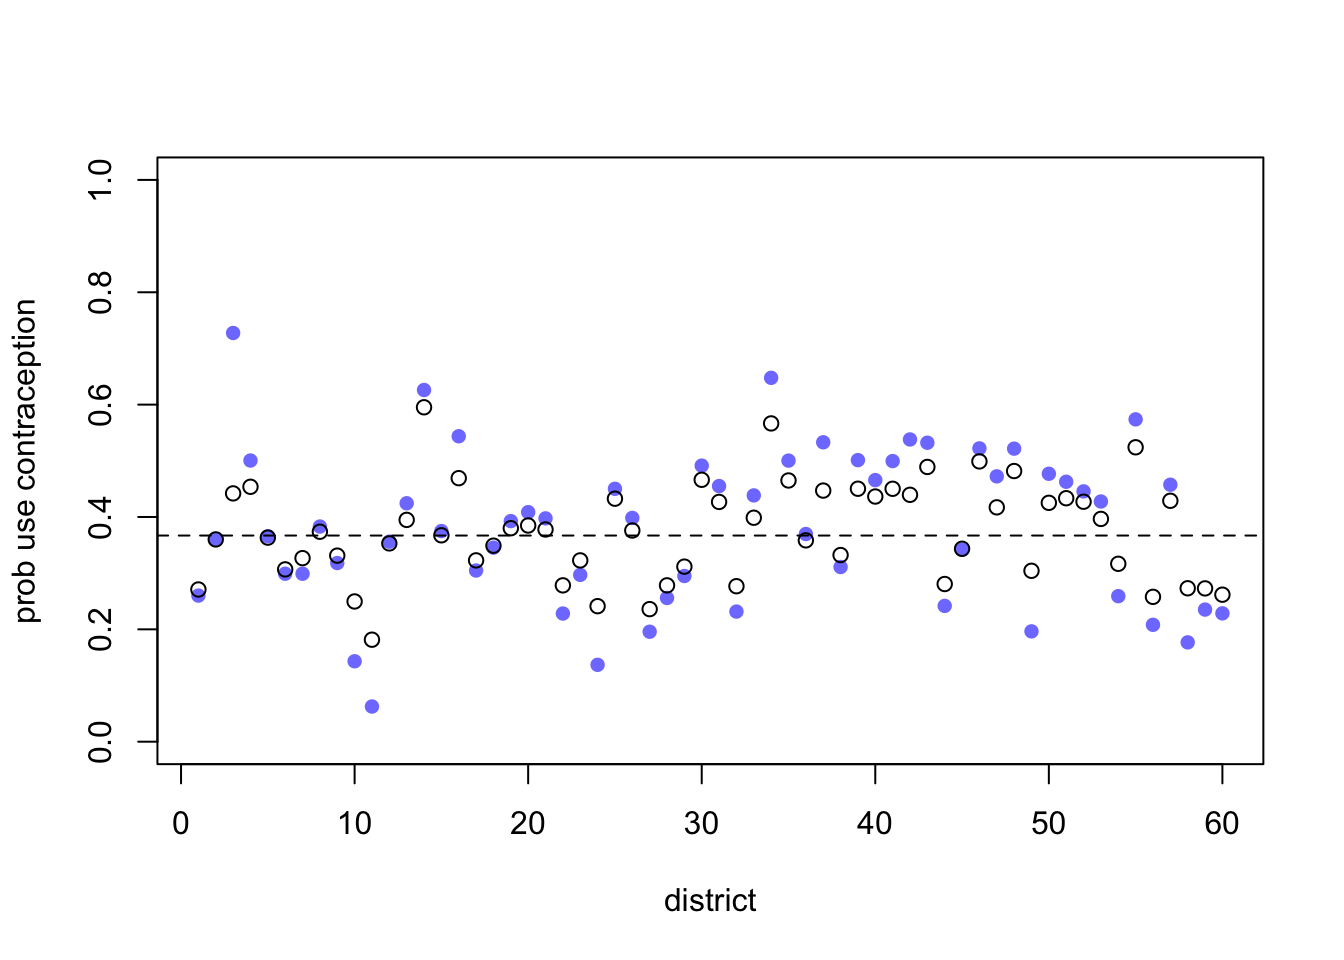
\includegraphics{rethinkingINLA_HW8_files/figure-latex/8.2.3 plot rethinking-1.pdf}

\hypertarget{plot-inla}{%
\subsubsection{plot inla}\label{plot-inla}}

\url{https://people.bath.ac.uk/jjf23/inla/oneway.html}

\url{https://people.bath.ac.uk/jjf23/brinla/reeds.html}

\textbf{posterior mean for each district a for the idex fixed effect
model m2.1:}

\begin{Shaded}
\begin{Highlighting}[]
\CommentTok{# m2.2.i$summary.fixed[[1]] would gives us the summary we want but not in the response scale, we need to  transform it using the inverse logit }

\NormalTok{inverse_logit <-}\StringTok{ }\ControlFlowTok{function}\NormalTok{ (x)\{}
\NormalTok{    p <-}\StringTok{ }\DecValTok{1}\OperatorTok{/}\NormalTok{(}\DecValTok{1} \OperatorTok{+}\StringTok{ }\KeywordTok{exp}\NormalTok{(}\OperatorTok{-}\NormalTok{x))}
\NormalTok{    p <-}\StringTok{ }\KeywordTok{ifelse}\NormalTok{(x }\OperatorTok{==}\StringTok{ }\OtherTok{Inf}\NormalTok{, }\DecValTok{1}\NormalTok{, p)}
\NormalTok{    p \}}

\CommentTok{#inla.tmarginal : apply inverse logit to all district marginals }
\CommentTok{#inla.zmarginal : summary of the logit-transformed marginals }
\CommentTok{# we eliminate the first element of this list, the intercept.}
\NormalTok{m2.}\FloatTok{1.}\NormalTok{i.fix<-}\StringTok{ }\KeywordTok{lapply}\NormalTok{(m2.}\FloatTok{1.}\NormalTok{i}\OperatorTok{$}\NormalTok{marginals.fixed, }\ControlFlowTok{function}\NormalTok{ (x) }\KeywordTok{inla.zmarginal}\NormalTok{( }\KeywordTok{inla.tmarginal}\NormalTok{ (inverse_logit, x )))[}\OperatorTok{-}\DecValTok{1}\NormalTok{]}
\end{Highlighting}
\end{Shaded}

\textbf{posterior mean for each district a for the varying intercept
model m2.2:}

\begin{Shaded}
\begin{Highlighting}[]
\CommentTok{# m2.2.i$summary.random[[1]] would gives us the summary we want but not in the response scale, we need to  transform it using the inverse logit }

\CommentTok{#inla.tmarginal : apply inverse logit to all district marginals }
\CommentTok{#inla.zmarginal : summary of the logit-transformed marginals }
\NormalTok{m2.}\FloatTok{2.}\NormalTok{i.rand<-}\StringTok{ }\KeywordTok{lapply}\NormalTok{(m2.}\FloatTok{2.}\NormalTok{i}\OperatorTok{$}\NormalTok{marginals.random}\OperatorTok{$}\NormalTok{district_id, }\ControlFlowTok{function}\NormalTok{ (x) }\KeywordTok{inla.zmarginal}\NormalTok{( }\KeywordTok{inla.tmarginal}\NormalTok{ (inverse_logit, x )))}
\end{Highlighting}
\end{Shaded}

\begin{Shaded}
\begin{Highlighting}[]
\CommentTok{# sapply(m2.2.i.rand, function(x) x[1]) extracts the first element (the mean) from the summary of the posterior of each district}
\NormalTok{m2.i.mean <-}\StringTok{ }\KeywordTok{bind_cols}\NormalTok{(}\DataTypeTok{district=} \DecValTok{1}\OperatorTok{:}\DecValTok{60}\NormalTok{,}\DataTypeTok{mean.m2.1=} \KeywordTok{unlist}\NormalTok{(}\KeywordTok{sapply}\NormalTok{(m2.}\FloatTok{1.}\NormalTok{i.fix, }\ControlFlowTok{function}\NormalTok{(x) x[}\DecValTok{1}\NormalTok{])), }\DataTypeTok{mean.m2.2=}\KeywordTok{unlist}\NormalTok{(}\KeywordTok{sapply}\NormalTok{(m2.}\FloatTok{2.}\NormalTok{i.rand, }\ControlFlowTok{function}\NormalTok{(x) x[}\DecValTok{1}\NormalTok{])))}

\NormalTok{m2.}\FloatTok{2.}\NormalTok{i.abar <-}\StringTok{ }\KeywordTok{inla.zmarginal}\NormalTok{( }\KeywordTok{inla.tmarginal}\NormalTok{ (inverse_logit, m2.}\FloatTok{2.}\NormalTok{i}\OperatorTok{$}\NormalTok{marginals.fixed[[}\StringTok{"(Intercept)"}\NormalTok{]] ))}
\end{Highlighting}
\end{Shaded}

\begin{verbatim}
## Mean            0.370149 
## Stdev           0.0193718 
## Quantile  0.025 0.331663 
## Quantile  0.25  0.357164 
## Quantile  0.5   0.37022 
## Quantile  0.75  0.383175 
## Quantile  0.975 0.407995
\end{verbatim}

\begin{Shaded}
\begin{Highlighting}[]
\NormalTok{m2.i.district.plot <-}\StringTok{ }\KeywordTok{ggplot}\NormalTok{() }\OperatorTok{+}
\StringTok{  }\KeywordTok{geom_point}\NormalTok{(}\DataTypeTok{data=}\NormalTok{ m2.i.mean, }\KeywordTok{aes}\NormalTok{(}\DataTypeTok{x=}\NormalTok{ district, }\DataTypeTok{y=}\NormalTok{ mean.m2}\FloatTok{.1}\NormalTok{), }\DataTypeTok{color=} \StringTok{"blue"}\NormalTok{, }\DataTypeTok{alpha=} \FloatTok{0.5}\NormalTok{)}\OperatorTok{+}
\StringTok{  }\KeywordTok{geom_point}\NormalTok{(}\DataTypeTok{data=}\NormalTok{ m2.i.mean, }\KeywordTok{aes}\NormalTok{(}\DataTypeTok{x=}\NormalTok{ district, }\DataTypeTok{y=}\NormalTok{ mean.m2}\FloatTok{.2}\NormalTok{), }\DataTypeTok{color=} \StringTok{"black"}\NormalTok{, }\DataTypeTok{alpha=} \FloatTok{0.5}\NormalTok{, }\DataTypeTok{shape=} \DecValTok{1}\NormalTok{)}\OperatorTok{+}
\StringTok{  }\KeywordTok{geom_hline}\NormalTok{(}\DataTypeTok{yintercept=}\NormalTok{m2.}\FloatTok{2.}\NormalTok{i.abar[[}\DecValTok{1}\NormalTok{]], }\DataTypeTok{linetype=}\StringTok{'longdash'}\NormalTok{) }\OperatorTok{+}
\StringTok{  }\KeywordTok{ylim}\NormalTok{(}\DecValTok{0}\NormalTok{,}\DecValTok{1}\NormalTok{)}\OperatorTok{+}
\StringTok{  }\KeywordTok{labs}\NormalTok{(}\DataTypeTok{y =} \StringTok{"prob use contraception"}\NormalTok{)}\OperatorTok{+}
\StringTok{  }\KeywordTok{theme_bw}\NormalTok{()}
  

\NormalTok{m2.i.district.plot}
\end{Highlighting}
\end{Shaded}

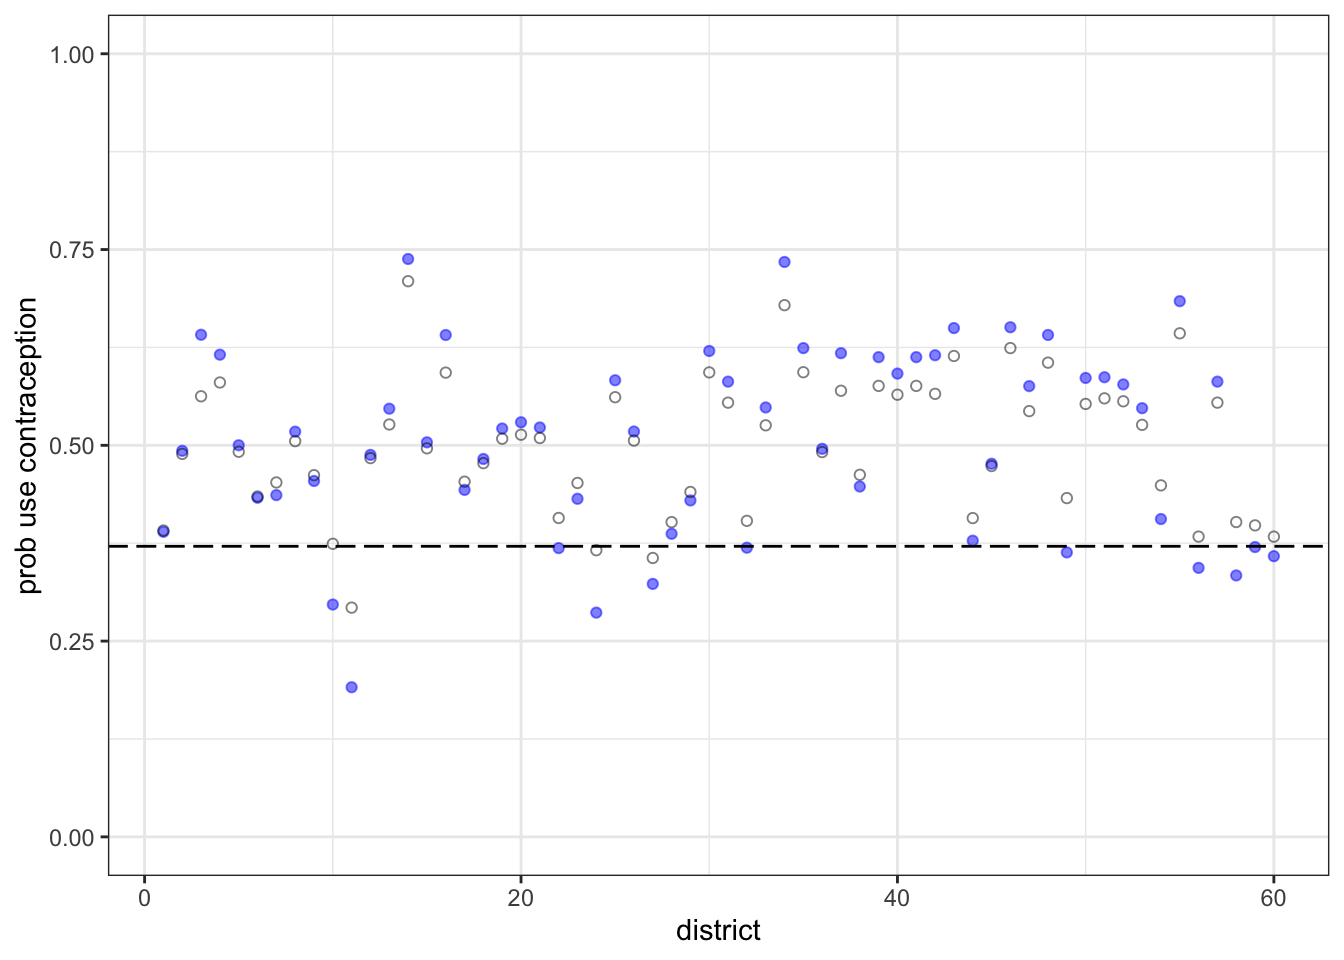
\includegraphics{rethinkingINLA_HW8_files/figure-latex/8.2.3 plot inla-1.pdf}

The blue points are the fixed estimations. The open points are the
varying effects. As you'd expect, they are shrunk towards the mean (the
dashed line). Some are shrunk more than others. The third district from
the left shrunk a lot. Let's look at the sample size in each district:

\begin{Shaded}
\begin{Highlighting}[]
 \KeywordTok{table}\NormalTok{(d}\OperatorTok{$}\NormalTok{district_id)}
\end{Highlighting}
\end{Shaded}

\begin{verbatim}
## 
##   1   2   3   4   5   6   7   8   9  10  11  12  13  14  15  16  17  18  19  20  21  22  23  24  25  26  27  28  29  30  31  32  33  34  35  36 
## 117  20   2  30  39  65  18  37  23  13  21  29  24 118  22  20  24  47  26  15  18  20  15  14  67  13  44  49  32  61  33  24  14  35  48  17 
##  37  38  39  40  41  42  43  44  45  46  47  48  49  50  51  52  53  54  55  56  57  58  59  60 
##  13  14  26  41  26  11  45  27  39  86  15  42   4  19  37  61  19   6  45  27  33  10  32  42
\end{verbatim}

District 3 has only 2 women sampled. So it shrinks a lot. There are
couple of other districts, like 49 and 54, that also have very few women
sampled. But their fixed estimates aren't as extreme, so they don't
shrink as much as district 3 does. All of this is explained by partial
pooling, of course.

\hypertarget{section-2}{%
\section{3.}\label{section-2}}

I don't really care about ordered categorical data so i'm going to skip
exercise 3.

\end{document}
